%!TEX root = ../thesis.tex

\subsection{Sweepcycle algorithm}
\thispagestyle{plain}
\label{ss:sweep}
The first step of our algorithm is executing a sweepcycle algorithm inspired by the sweepcycle algorithm by Fusy \cite{Fusy2006}. We use $\C$ to indicate the current sweep cycle. We shrink $\C$ by updating it with interior paths.
The algorithm finishes when $\C$ has no more interior vertices. When the algorithm finishes, it has produced a regular edge labeling.
One of the nicest things about the regular edge labeling is Lemma \ref{lm:sweep:NoTwoSplitsAboveEachOther}.
This lemma states that we can not have the fan handle of a large topfan after a split vertex on a so-called bottom path.

During the algorithm we maintain several invariants on $\C$. The first four are equivalent to those imposed by Fusy. The final invariant is new and allows us to prove Lemma \ref{lm:sweep:NoTwoSplitsAboveEachOther}.

\begin{invariants}
  \itemsep=-4pt
  \item \label{i:uni:SWandSE} The cycle $\C$ contains the two edges $\pS \pW$ and $\pS \pE$.
  \item \label{i:uni:noChords} $\cpath$ has no chords.
  \item \label{i:uni:intVertCond} The inner vertex condition holds for all vertices in the exterior of $C$.
  \item \label{i:uni:redOutgoing} Every non-pole vertex on the sweepcycle has a red outgoing edge.
  \item \label{i:uni:no2Chords} $\C\sm{\pS}$ has no separating 2-chords that do not use $\pS$.
\end{invariants}

We initialize the sweepcycle $\C$ with the outer cycle of $\ext G$.
We denote the vertices of the sweepcycle $\C$ by $\pS, v_1 = \pW, v_2, \ldots v_{n-1}, v_n = \pE, \pS$.
We repeatedly consider the path $\cpath$.
In which case we order it from $\pW$ to $\pE$. That the edges $\pS \pW$ and $\pS \pE$ are always in $\C$ is a result of Invariant \ref{i:uni:SWandSE}.


Each update of the sweepcycle consists of the following three steps.
\begin{enumerate}
  \itemsep=-4pt
  \item Take the right neighbor walk of a subpath of $\cpath$ to get the \emph{candidate path} $P$.
  \item Evade violating chords on $P$ to get the \emph{updating path} $P'$.
  \item Update the sweepcycle with $P'$.
\end{enumerate}

We repeat these steps until the sweepcycle does not contain anymore interior vertices. At which point we can terminate the algorithm by coloring the edges of the cycle $\C$ blue and its interior edges red.

\subsubsection{Find the right neighbor path}
  Recall we denote all the vertices of $\cpath$ by $\pW =  v_1   v_2   \ldots v_{n-1}   v_n = \pE$.
  Suppose they are all adjacent to $S$, then any vertex still in the interior of $\C$ would lie in a separating triangle of $G$. So we have no interior vertices and hence we can terminate the algorithm as described in Section~\ref{sss:terminating}.
  In the remainder we assume some vertices from $\cpath$ are not adjacent to $\pS$.

  Since $\cpath$ has some vertices incident to $\pS$ (at least $\pW and \pE$) and some that are not, we can consider maximal subpaths of $\cpath$ consisting of vertices adjacent to $\pS$.
  We denote by $v_i$ the last vertex of first maximal subpath of vertices adjacent to $\pS$ and by $v_j$ the first vertex of the second maximal subpath.
  As candidate path $P$ we take the right neighbor path of $\cpath|_{v_i, v_j}$. This right neighbor path does indeed exist since all internal vertices of $\cpath|_{v_i, v_j}$ are interior vertices of $G$ and $\cpath$ has no violating chords by Invariants \ref{i:uni:noChords} and \ref{i:uni:no2Chords}.
  This situation is depicted in Figure~\ref{fig:sweep:noIrregularity}.

\subsubsection{Evading violating chords}
  Recall that a violating chords on the candidate path $P$ can be one of the following two things:
  \begin{enumerate}
    \itemsep=-4pt
    \item Chords
    \item Separating 2-chords
  \end{enumerate}

  The \emph{middle} vertex of a $2$-chord is the only internal vertex of that $2$-chord (seen as a path).
  All violating chords are on the right of the candidate path due to Lemma \ref{lm:right:neighbourwalkChordFree} (no chords on the left) and Lemma \ref{lm:right:neighbourwalkNoInteriorVertex} (no separating 2-chords on the left).

  Before we can show how to evade these structures, we first introduce more notation. We orient $P$ from $v_i \in \C$ (the vertex closest to $\pW$) to $v_j \in \C$ (the vertex closest to $\pE$) and denote its vertices by $p_1 \ldots p_r$.
  The \emph{index} of a vertex $p_m \in P$ is its position in the path, that is, the index of $p_m$ is $m$.
  The \emph{start index} of an violating chord $C$ is the index of the first vertex in $P$ that is also in $C$. Similarly, the \emph{end index} is the index of the last vertex in $P$ that is also in $C$.
  The \emph{range} of an violating chord is given by its start and end index. We update the sweepcycle with some \emph{update path} $P'$, depending on the violating chords we find on the candidate path $P$. This update is described in Section~\ref{sss:sweep:update}.

  While describing how the updating path $P$ depends on the violating chords of $P$ we show that the following two lemmas hold in every case.

  \begin{lemma}
    The updating path has no violating chords
    \label{lm:sweep:augNoIregularity}
  \end{lemma}

  \begin{lemma}
    \label{lm:sweep:noConnectingIregularity}
    There are no violating chords, not containing $\pS$ as middle vertex, with one endpoint on the sweepcycle $\C$ and one endpoint on the updating path $P'$.
  \end{lemma}

  \mypar{We have no violating chord}
    When $P$ has no violating chords, we update the sweepcycle with the entire candidate path $P$.
    In this case the update path $P'$ is equal to $P$.

    $P'$ has no violating chord by the definition of this case. Moreover, there are no violating chords with one endpoint on $P'$ and one endpoint on $\C$ since $v_i$ and $v_j$ are both adjacent to $\pS$, so we can not have any chords and any $2$-chords must have $\pS$ as middle vertex.
    \begin{figure}[t]
      \centering
      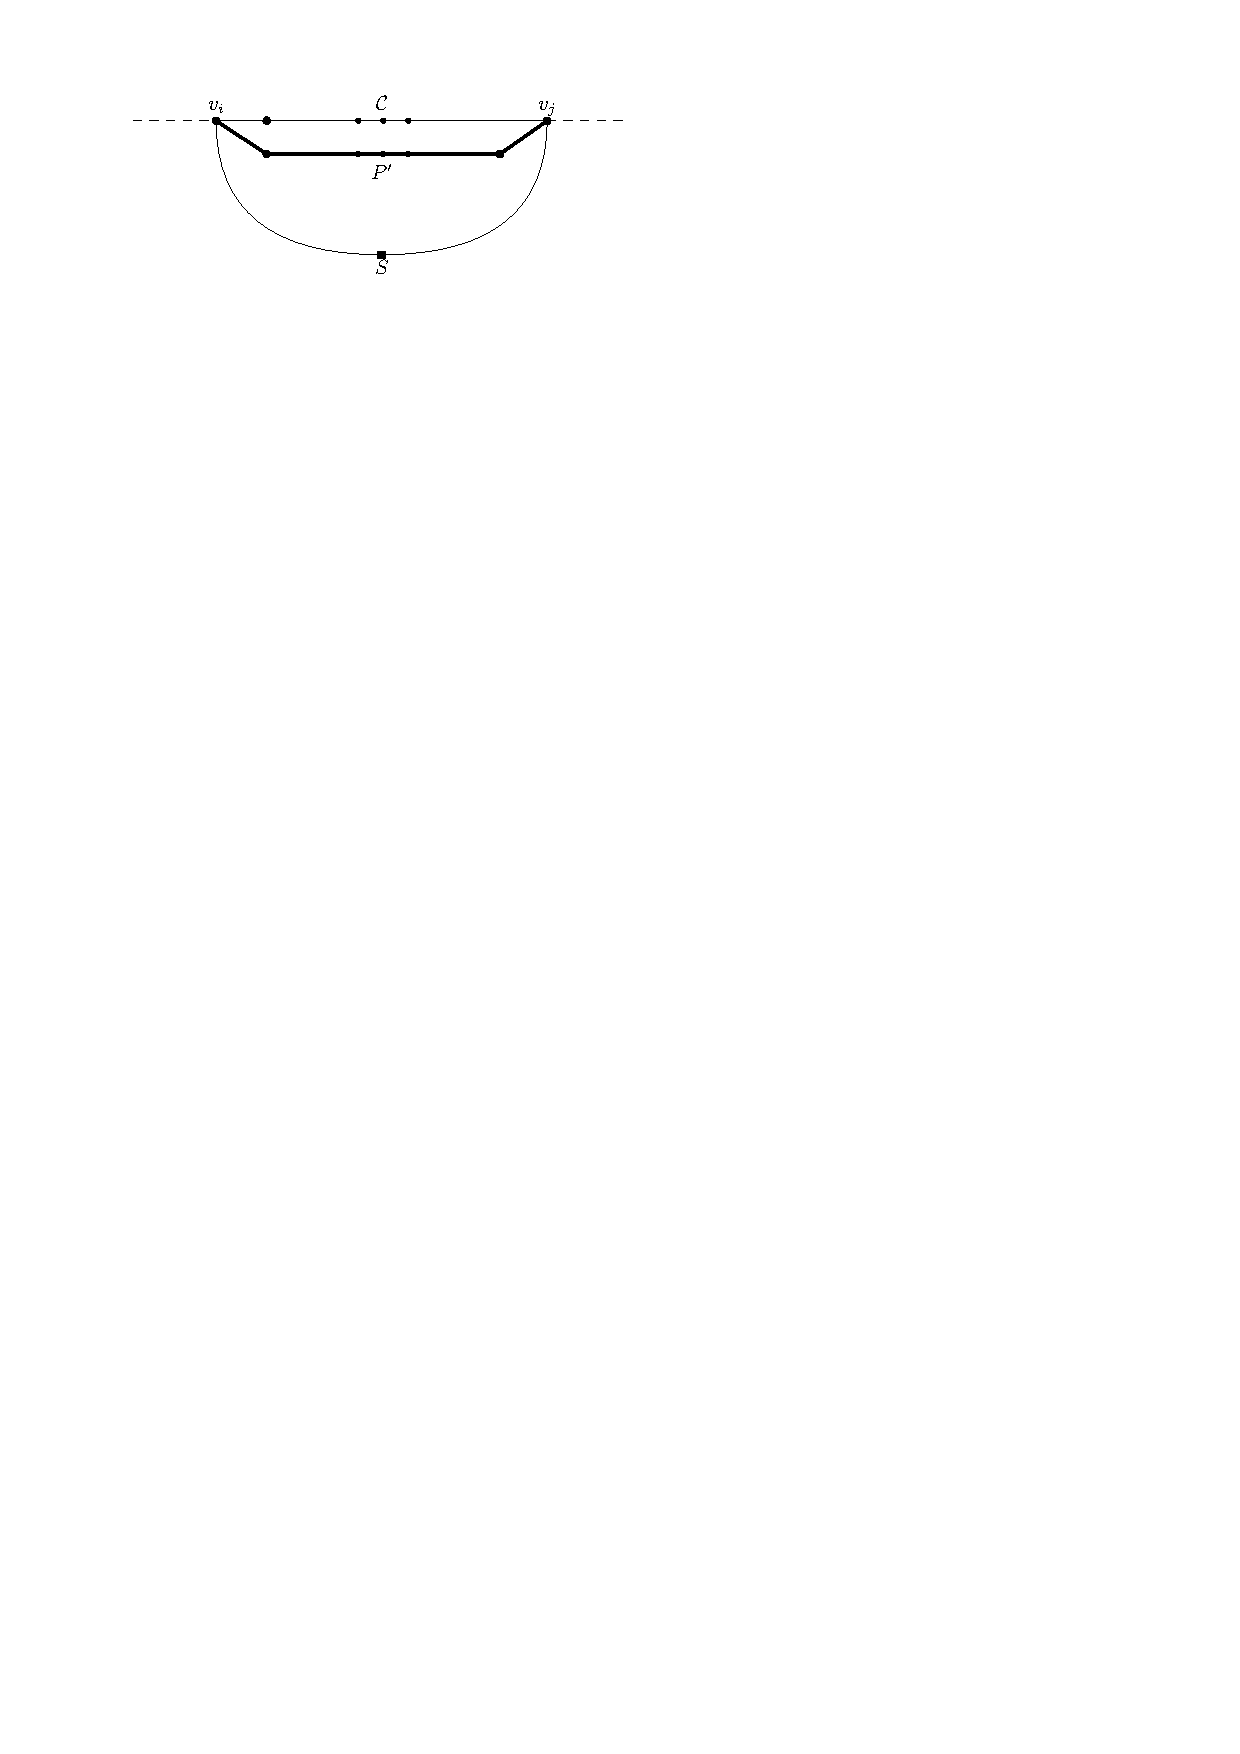
\includegraphics[scale=1]{unifiedAlgo/img/sweep/cases/noIrregularity}
      \caption{Updating path when $P$ contains no violating chord.}
      \label{fig:sweep:noIrregularity}
    \end{figure}

  \mypar{We have a chord on $\mathbf{P}$}
    Note that we can not have a chord incident to one of the exterior vertices of the candidate path $P$, that is $p_1$ or $p_r$, since any such chord would violate Invariant \ref{i:uni:no2Chords} of $\C$ as can be seen in Figure~\ref{fig:sweep:noChordOnExteriorVertex}.

    \begin{figure}[b]
      \centering
      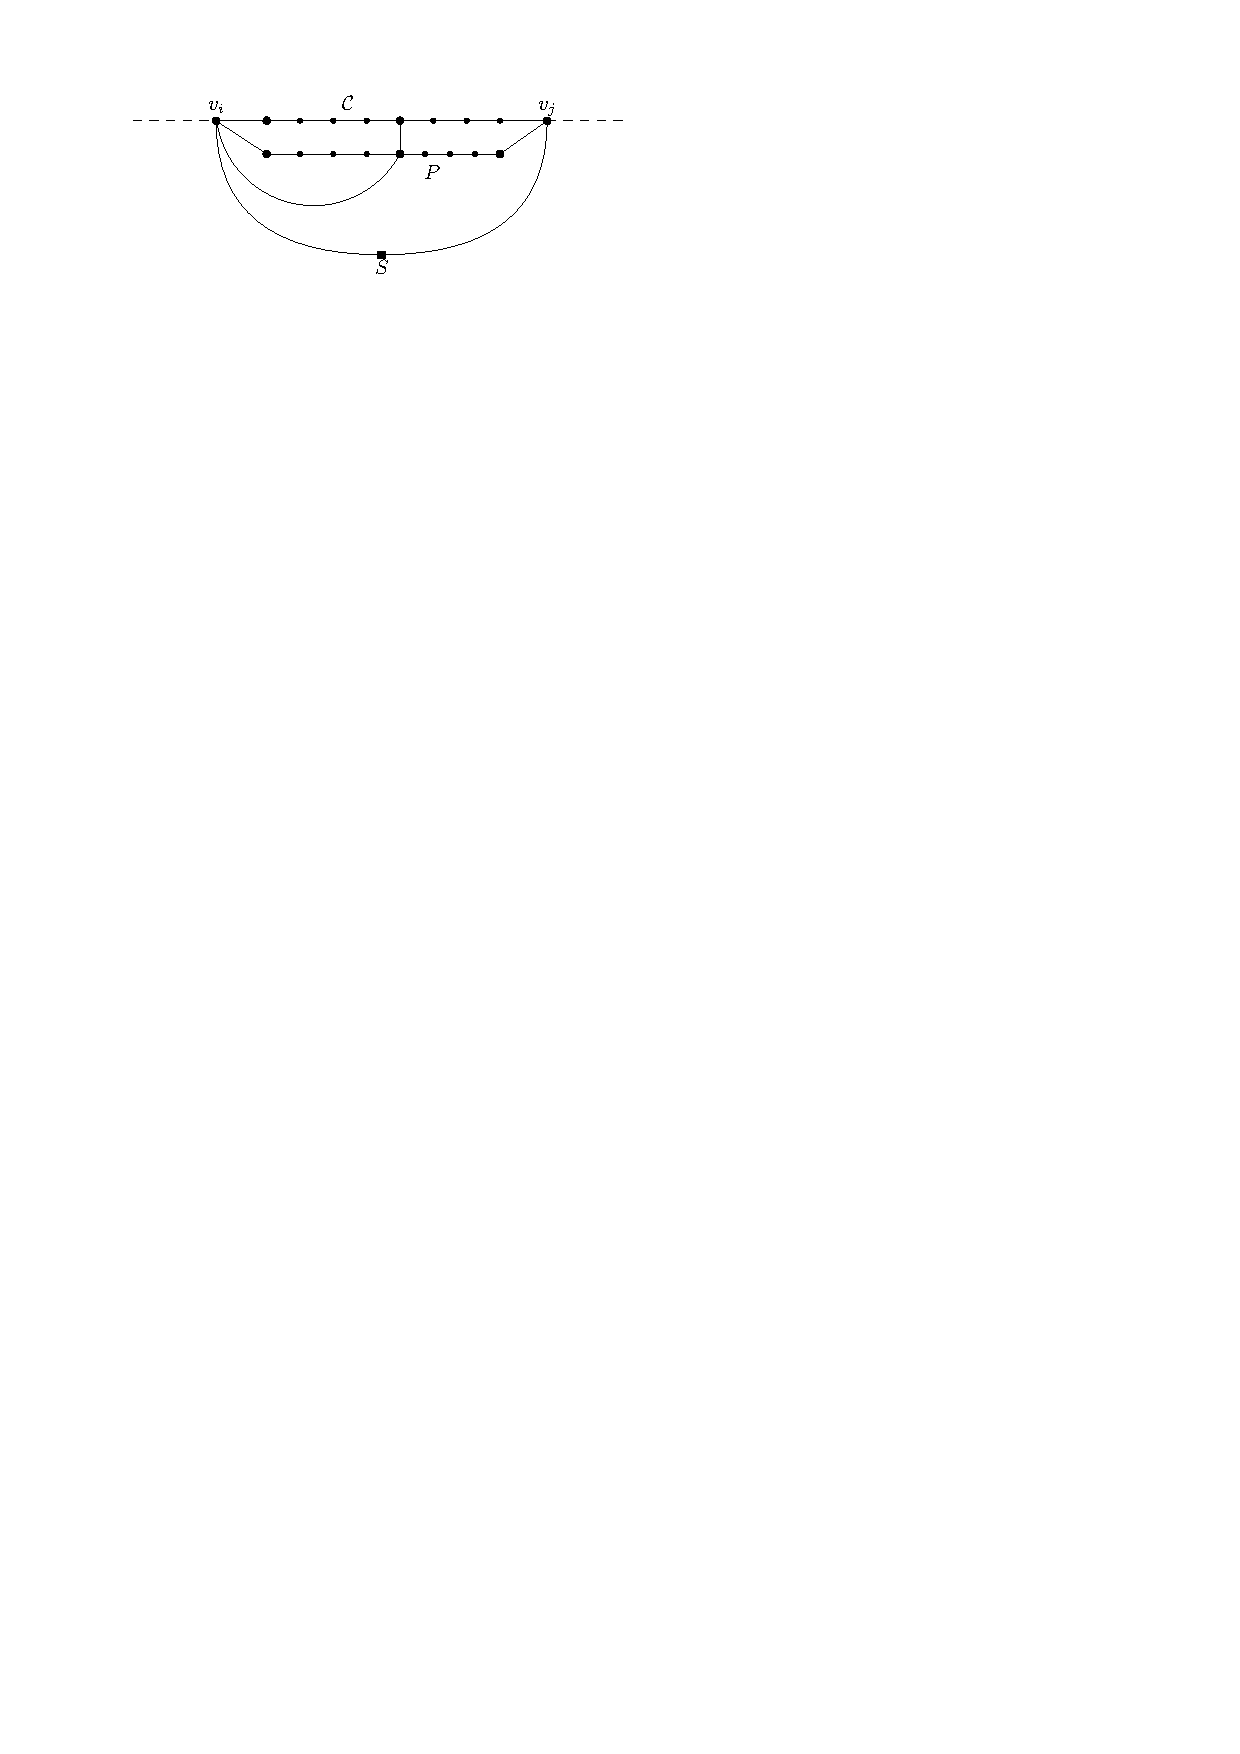
\includegraphics[scale=1]{unifiedAlgo/img/sweep/noChordOnExtriorVertex.pdf}
      \caption{Hypothetical situation where $P$ would have a chord on an exterior vertex.}
      \label{fig:sweep:noChordOnExteriorVertex}
    \end{figure}

    We identify the chords by their ranges. Of the chords with the smallest end index $m$ we consider the one with the largest start index $n$. We denote this chord by $C$.
    Note that this chord can not contain any other chords since such a chord would have either a large start index or a smaller end index.
    The way in which we find this chord $C$ is illustrated in Figure~\ref{fig:sweep:chordsOnCandidatePath}.

    \begin{figure}[t]
      \centering
      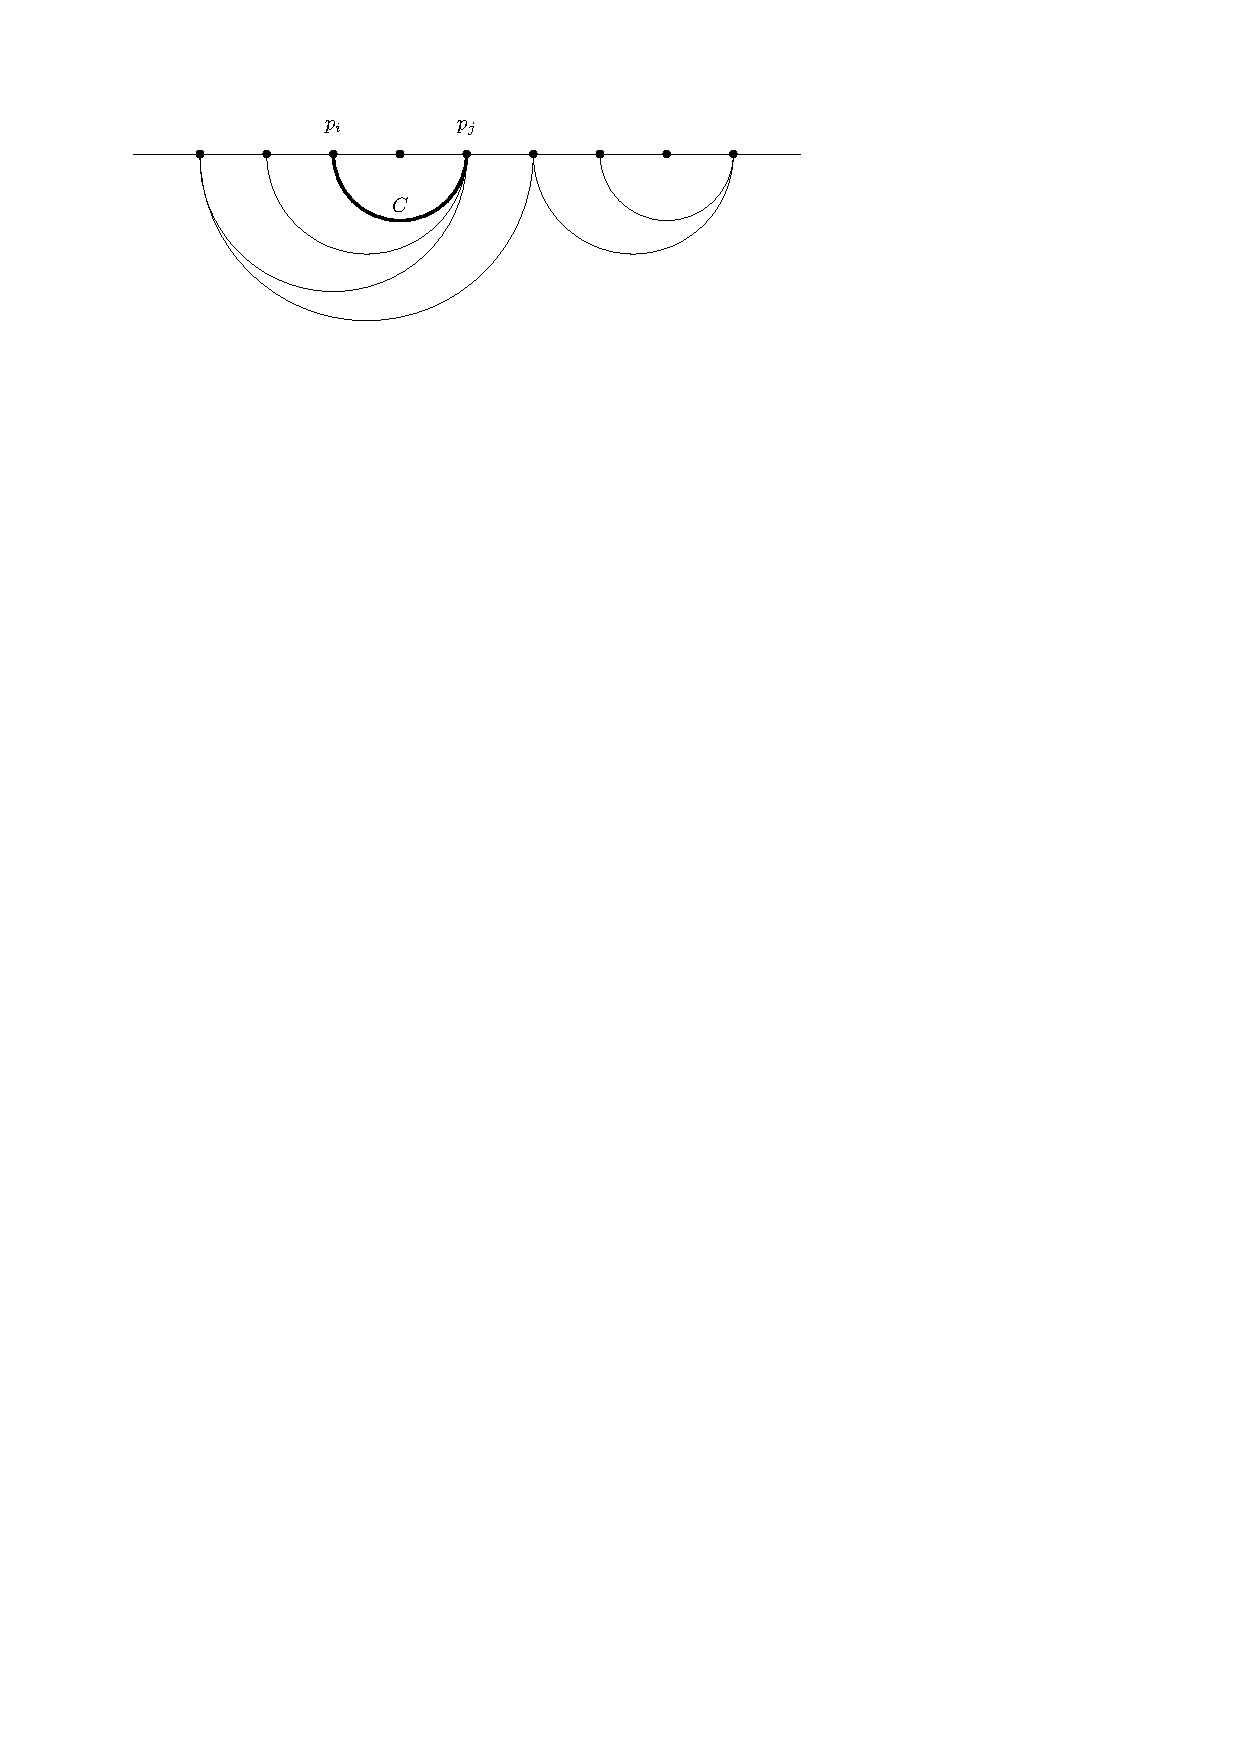
\includegraphics[scale=1]{unifiedalgo/img/sweep/chordsOnCandidatePath}
      \caption{Finding the chord $C$.}
      \label{fig:sweep:chordsOnCandidatePath}
    \end{figure}

    What we do now depends on whether a separating 2-chord shows up in the interior of the chord concatenated to the candidate path $P|_{m, n} \oplus \rev{{C}}$.

    \emph{No separating 2-chord.}
      If there is no separating 2-chord in the interior of $P|_{i, j} \oplus \rev{{C}}$ we let $v_k$ be the shared neighbor in $\C$ of $p_{m}$ and $p_{m +1}$ and we let $v_\ell$ the shared neighbor in $\C$ of $p_{n -1}$ and $p_{n}$.
      The updating path $P'$ is the right neighbor path of $\cpath|_{v_k, v_\ell}$.
      See Figure~\ref{fig:sweep:chordUpdate}.

      $P'$ is entirely inside a chord containing no more chords and thus can not contain a chord.
      Moreover, there are no separating $2$-chords on $P|_{p_m, p_n}$ so $P'$ can not have separating $2$-chords.
      So Lemma~\ref{lm:sweep:augNoIregularity} holds in this case.
      Any violating chord with one endpoint in $P'$ and one in $\C$ has to cross $v_k p_m p_n v_\ell$ so we can not have a chord and any 2-chord has $p_m$ or $p_n$ as middle vertex.
      But, with this restriction such a 2-chord can not be separating.
      So Lemma \ref{lm:sweep:noConnectingIregularity} also holds.

      \begin{figure}[!b]
        \centering
        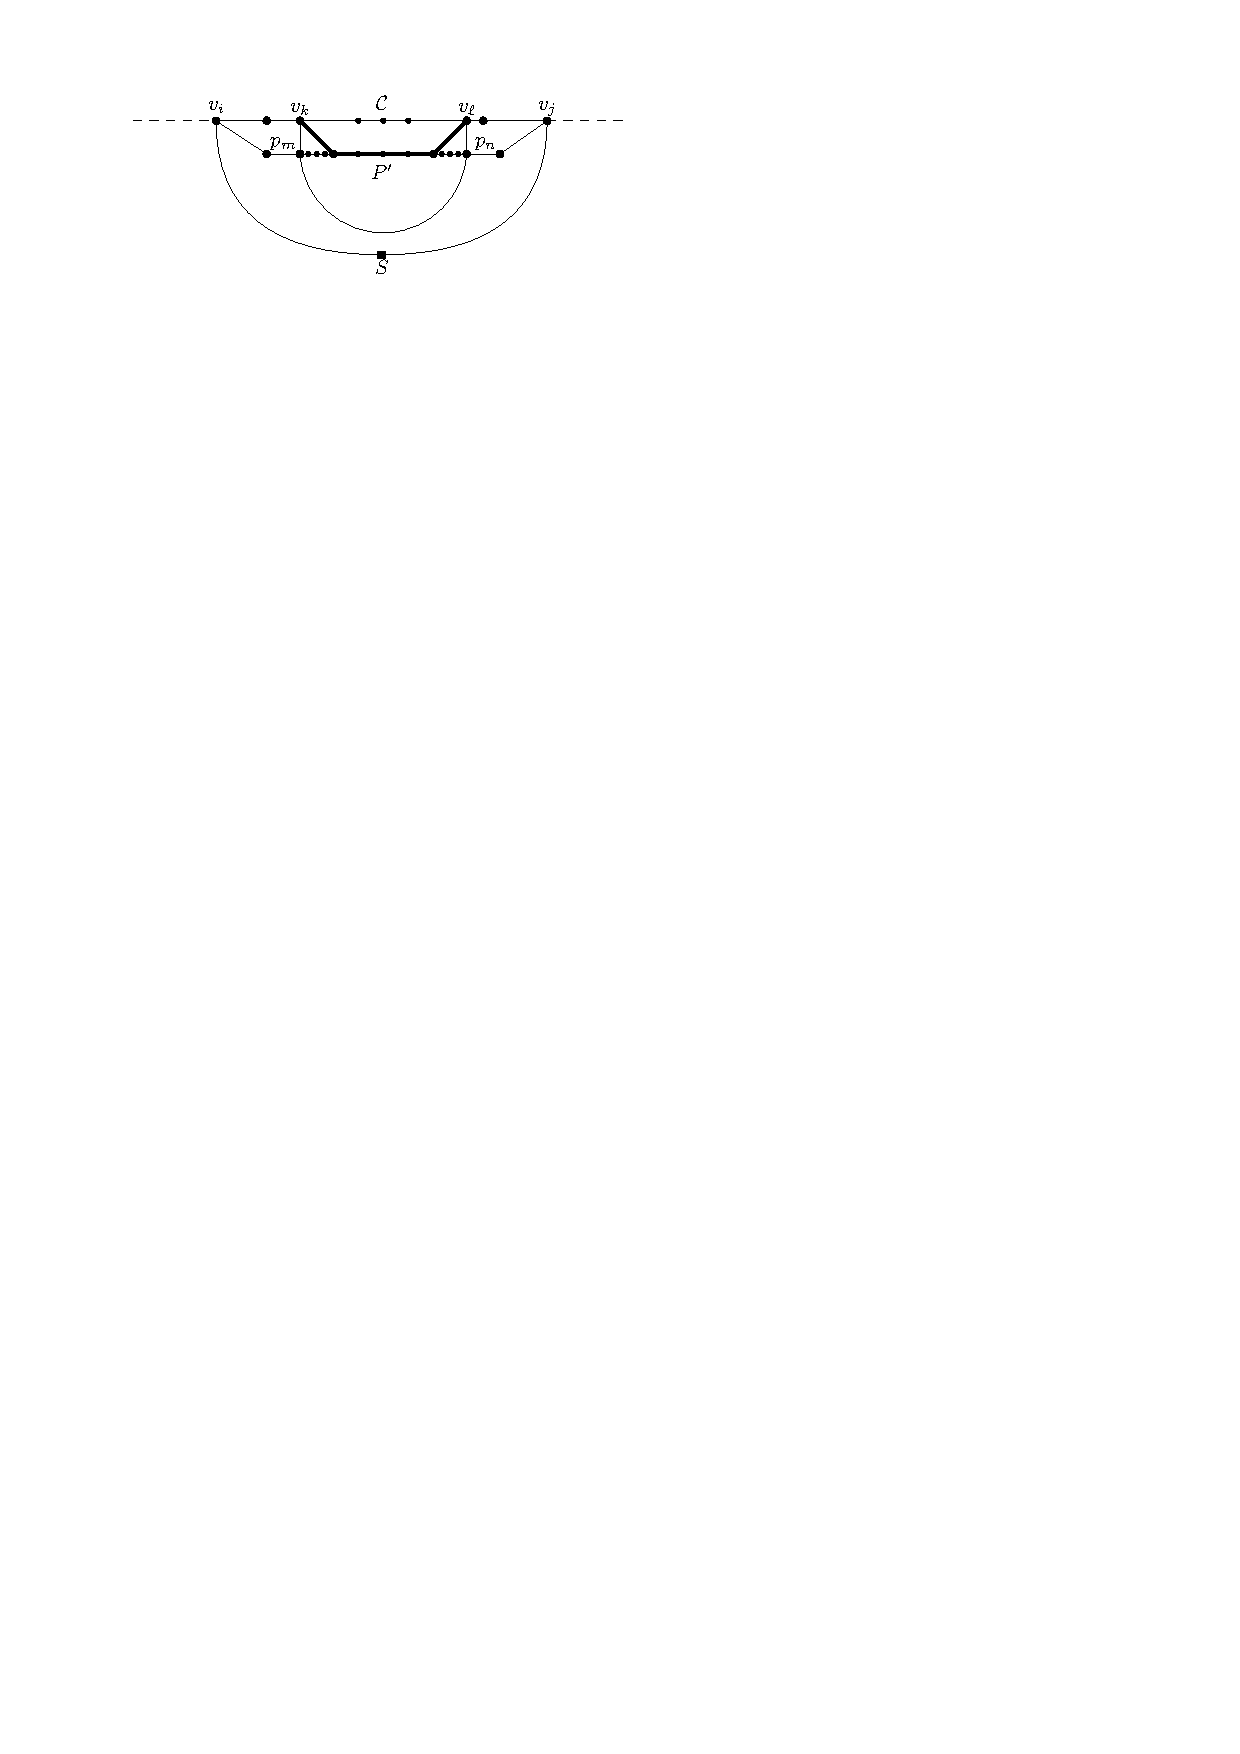
\includegraphics[scale=1]{unifiedAlgo/img/sweep/cases/chordUpdate}
        \caption{Updating path when $P$ has a chord not containing a separating 2-chord.}
        \label{fig:sweep:chordUpdate}
        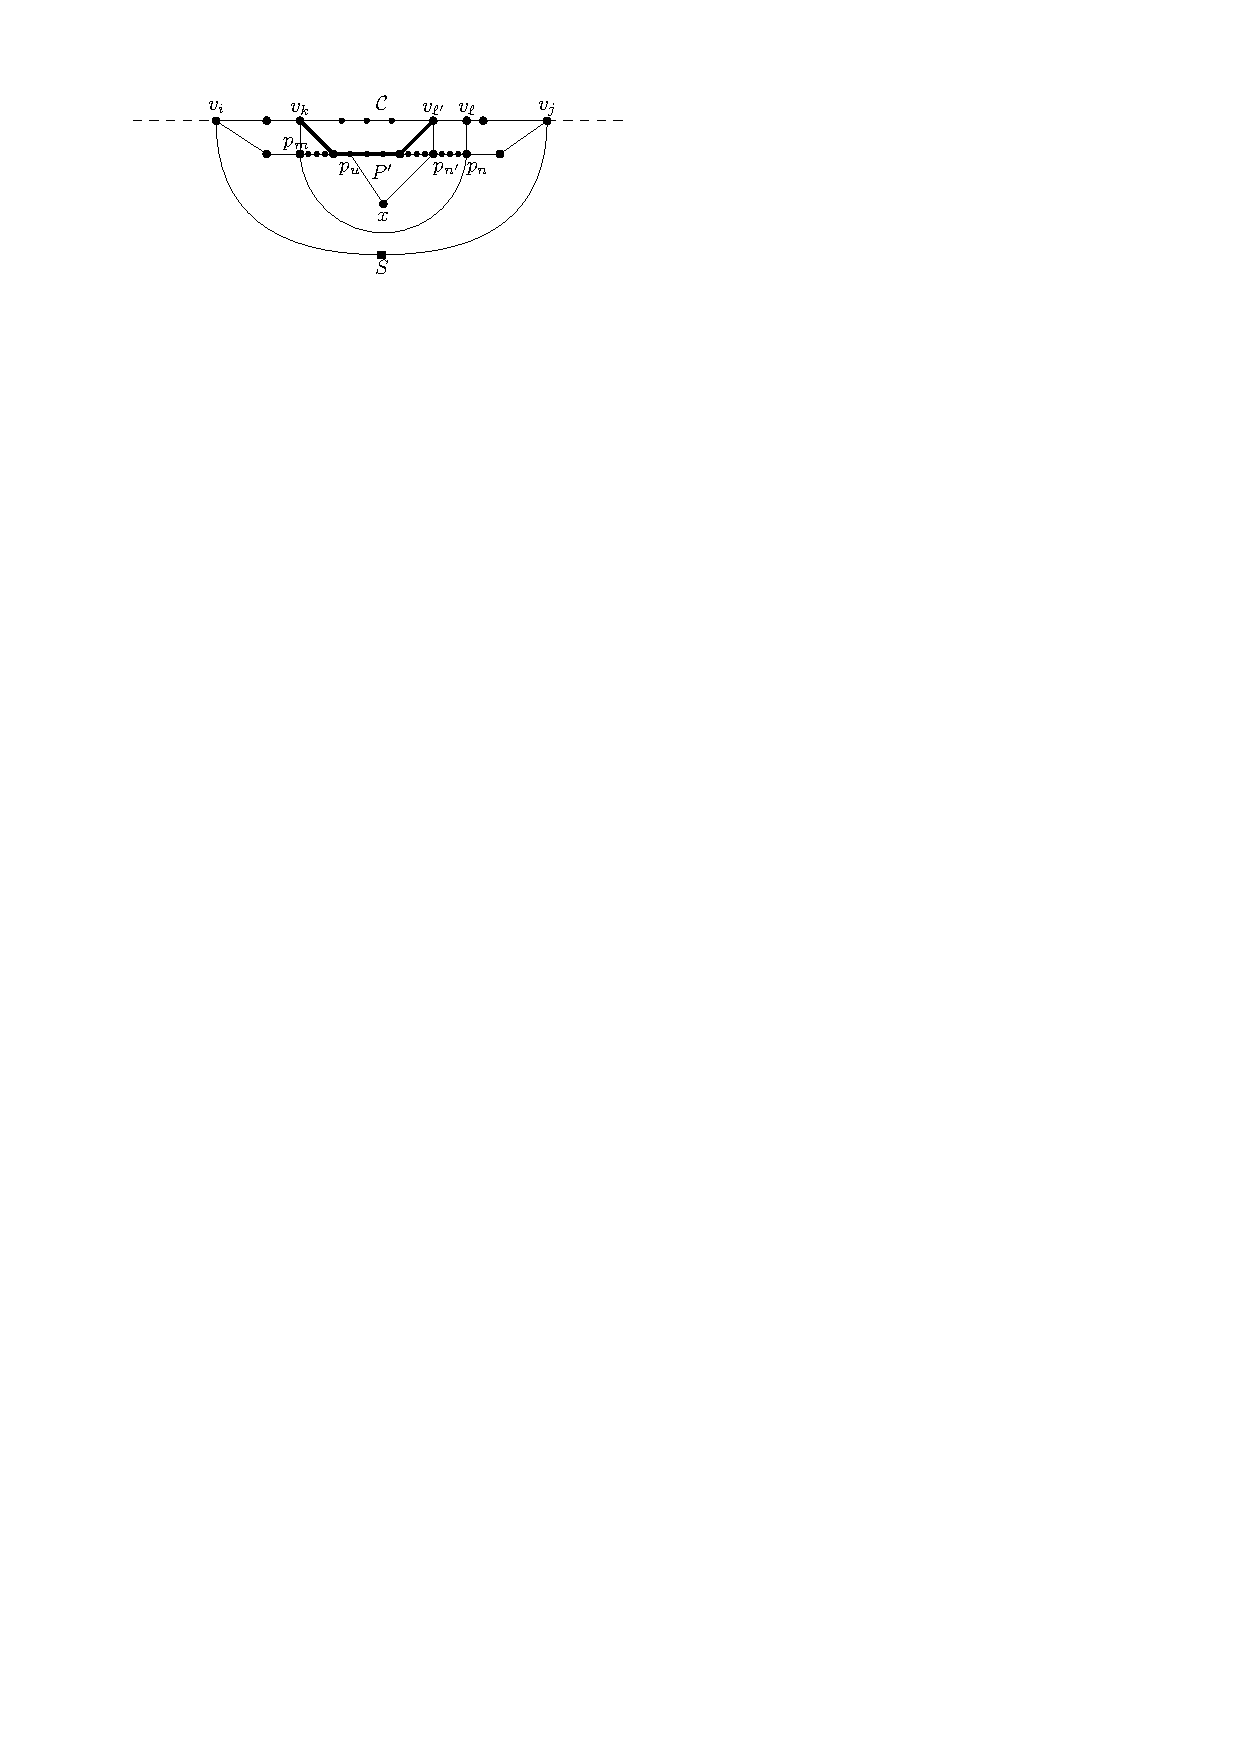
\includegraphics[scale=1]{unifiedAlgo/img/sweep/cases/2chordInChordUpdate}
        \caption{Updating path when $P$ has a chord containing at least one separating 2-chord.}
        \label{fig:sweep:2chordInChordUpdate}
      \end{figure}

    \emph{At least one separating 2-chord.}
      Let $n'$ be end index of the separating 2-chord with the lowest end index in the interior of $P|_{m, n} \oplus \rev{p_m p_n}$. And let $v_k$ be the shared neighbor on the sweepcycle of $p_{m}$ and $p_{m +1}$ and let $v_\ell$ and $v_{\ell'}$ be the shared neighbor on the sweepcycle  of $p_{n -1}$ and $p_{n}$ and of $p_{n' -1}$ and $p_{n'}$, respectively.
      Then the updating path $P'$ is the right neighbor path of $\cpath|_{v_k, v_{ell'}}$. See Figure~\ref{fig:sweep:2chordInChordUpdate}.

      $P'$ is entirely inside a chord containing no more chords and thus can not contain a chord. Moreover, $P'$ can not have a separating $2$-chord since we evaded the end of the first one ending.
      Just as in the above case we can not have any violating chord with one endpoint in $P'$ and one in $\C$ outside the containing chord $v_k p_m p_n v_\ell \oplus \rev \cpath |_{v_k, v_\ell}$.
      That leaves violating chords with the second endpoint inside the containing chord $v_k p_m p_n v_\ell \oplus \rev \cpath |_{v_k, v_\ell}$.
      Suppose that we have a separating $2$-chord, then this would have been a chord of $P$. This is in contradiction with $p_m p_n$ being a minimal chord.
      We also can not have a chord since this would break the cycle $P|_{p_m, p_n} \oplus p_n p_m$ .

  \mypar{Only separating 2-chords}
    In this case the candidate path $P$ has no chords, otherwise we would be in the above case. We split this case into two subcases, either we have a separating $2$-chord with $v_j$ as end vertex or we have only other separating $2$-chords.

    \emph{Any separating 2-chords with $v_j$ as end vertex.}
      We find the smallest separating 2-chord with $v_j$ as end vertex (i.e. the one with the highest start index). Say this separating $2$-chord has start index $i$.
      Let $v_k$ be the shared neighbor on the sweepcycle of $p_{m}$ and $p_{m +1}$. The updating path is the right neighbor path of $\cpath|_{v_k, v_j}$. See Figure~\ref{fig:sweep:pEBound}.

      $P'$ starts inside the separating $2$-chord adjacent to $v_j$ with the highest start index. $P'$ has no chords since $P$ already had none.
      However $P'$ can have separating $2$-chords that are not adjacent to $v_j$.
      If this is the case we find the $2$-chord with the lowest end index $n$.
      Let $v_\ell$ be the shared neighbor on the sweepcycle of $p_{n}$ and $p_{n-1}$.
      The updating path is the right neighbor path of $\cpath|_{v_k, v_\ell}$.

      We have no chords with one endpoint in $P'$ and one in $\C$ since these would have to break $v_j x p_m v_k \oplus \rev{P'}$ or be adjacent to $v_j$, which is in violation of Invariant \ref{i:uni:no2Chords}.
      Any $2$-chords with one endpoint in $P'$ and one in $\C$ would have $x$ or any vertex in $P$ as middle vertex.
      However, the first yields a $2$-chord of the candidate path with a higher start range, this is a contradiction.
      And the second gives a chord of $P$, this is in contradiction with the current case where $P$ has no chords.

    \begin{figure}[t]
      \centering
      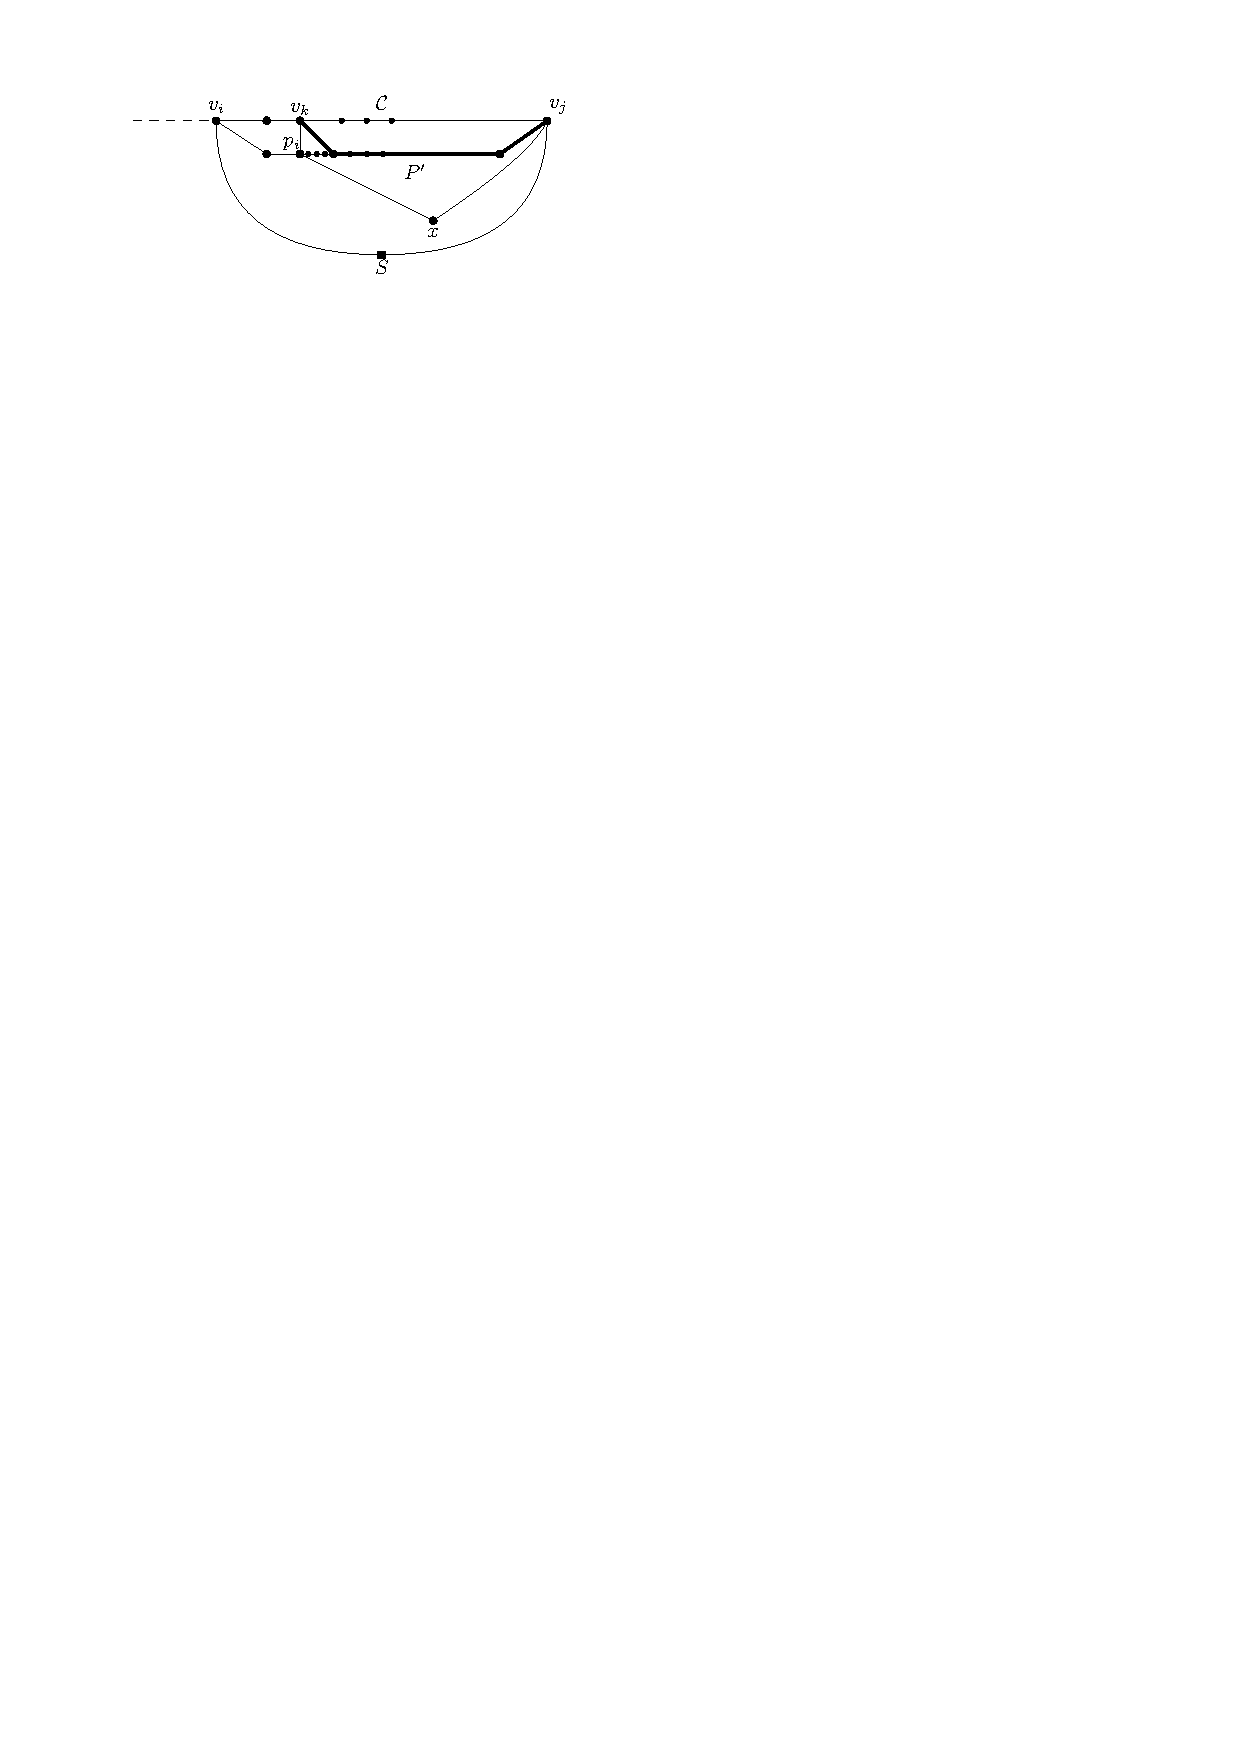
\includegraphics[scale=1]{unifiedAlgo/img/sweep/cases/pEBound}
      \caption{Updating path when $P$ has a separating 2-chord with $v_j$ as end vertex.}
      \label{fig:sweep:pEBound}
      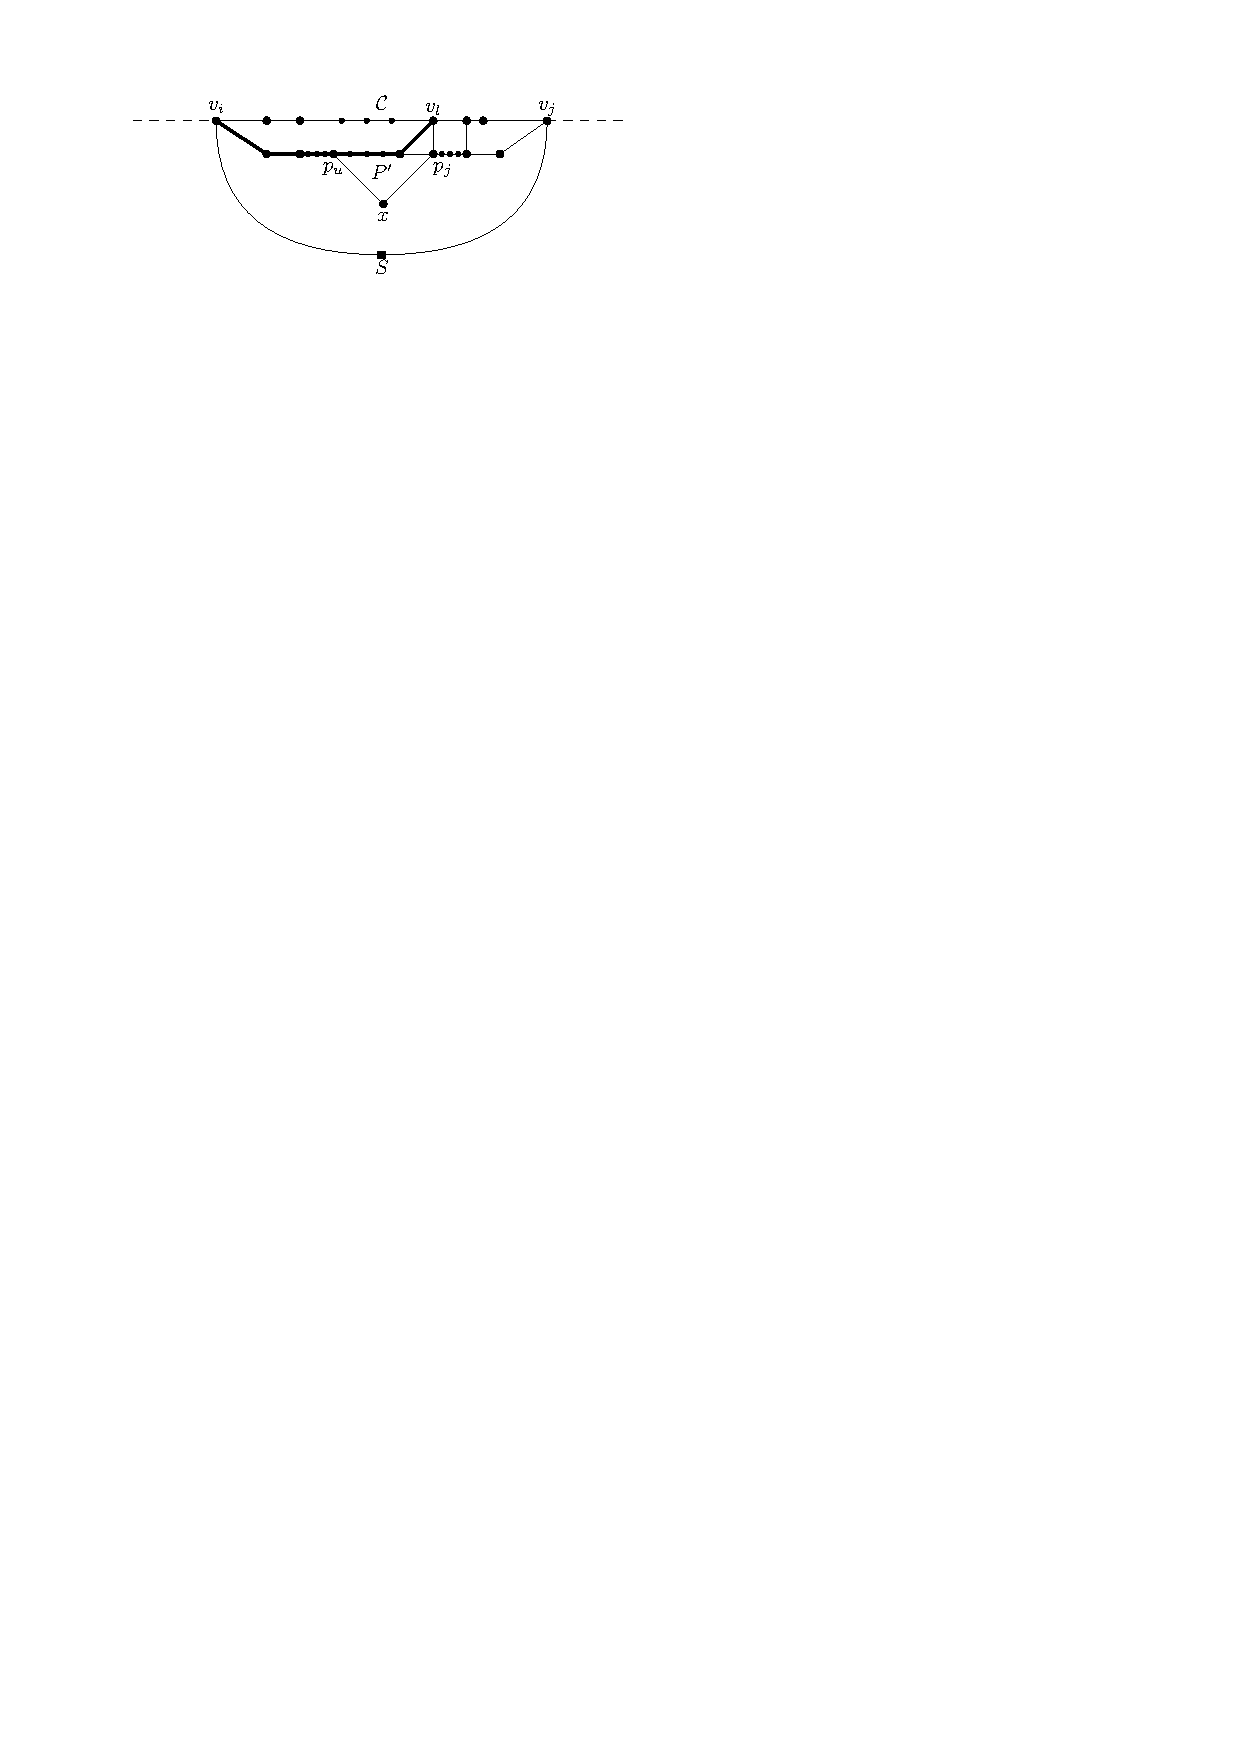
\includegraphics[scale=1]{unifiedAlgo/img/sweep/cases/free2chord}
      \caption{Updating path when $P$ has separating 2-chords none of which have $v_j$ as end vertex.}
      \label{fig:sweep:free2chord}
    \end{figure}

    \emph{Only other separating 2-chords}
      Find the $2$-chord with the lowest end index, say that this is $n$.
      Let $v_\ell$ be the shared neighbor on the sweepcycle of $p_{n}$ and $p_{n-1}$.
      The updating path is the right neighbor path of $\cpath|_{v_i, v_\ell}$. See Figure~\ref{fig:sweep:free2chord}.

      Any updating path stops before the end of a separating 2-chord and furthermore contains no chords since $P$ already did not.

      Any violating chord with one vertex in the updating path and the other on the old sweepcycle must end to the right of the updating path since the updating path starts at $v_i$, a vertex adjacent to $\pS$.
      Suppose that we have a separating $2$-chord then that would have been a chord of the candidate path. This is in contradiction with the assumption that the candidate path had no chords.
      We also have no chord since such a chord would violate Invariant \ref{i:uni:no2Chords} of the old sweepcycle. Furthermore, the second-to-last vertex of the updating path has no chords since it would break $v_\ell p_n x p_u$. (see Figure~\ref{fig:sweep:free2chord}).

\subsubsection{Updating}
  \label{sss:sweep:update}
  Once we found the updating path $P'$, we can update the sweepcycle with this path.  Let $p_a$ and $p_b$ indicate the two unique vertices of $P'$ that are also part of $\C$. We then let $\cpath|_{P'}$ denote the path $\cpath|_{p_a, p_b}$.
  In this section we describe how to update the sweepcycle with an updating path and we show that the update maintains all sweepcycle invariants (Lemma \ref{lm:sweep:updateMaintainsInvariants}).
  To execute the update we color all interior edge of $\cpath|_{P'} \oplus \rev{P'}$ red and orient them towards $\cpath_|{P'}$.
  We also color all edges of $\cpath|_{P'}$  blue and orient them from lower to higher induces.
  We then update the sweepcycle to $\C'$ by replacing $\cpath|_{P'}$ by $P'$ in $\C$.
  An example of the whole update for an updating path $P'$ can be seen in Figure~\ref{fig:sweep:update}.

  \begin{figure}[t]
      \centering
      \begin{subfigure}[b]{0.45 \textwidth}
          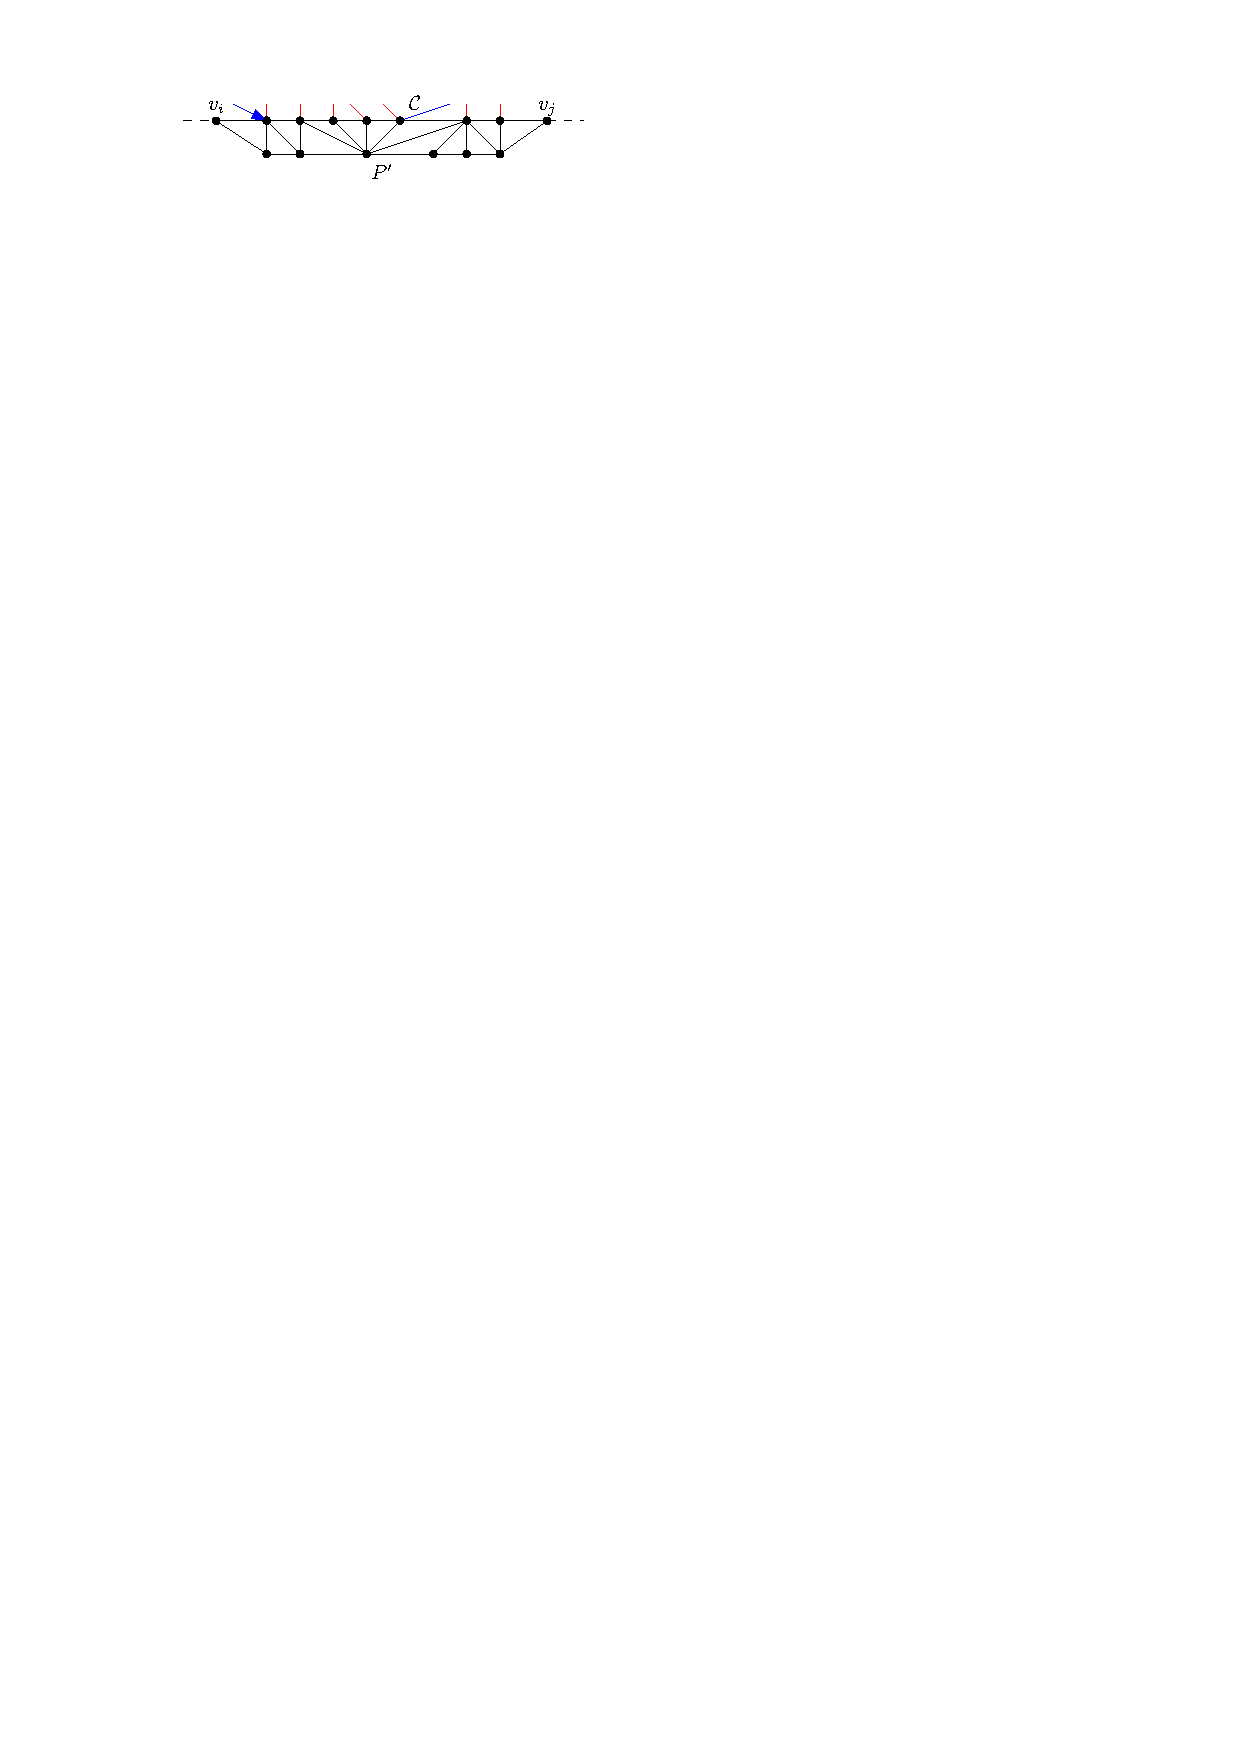
\includegraphics[width = \textwidth]{unifiedAlgo/img/sweep/updateBefore.pdf}
          \caption{Before.}
      \end{subfigure}
      ~
      \begin{subfigure}[b]{0.45 \textwidth}
          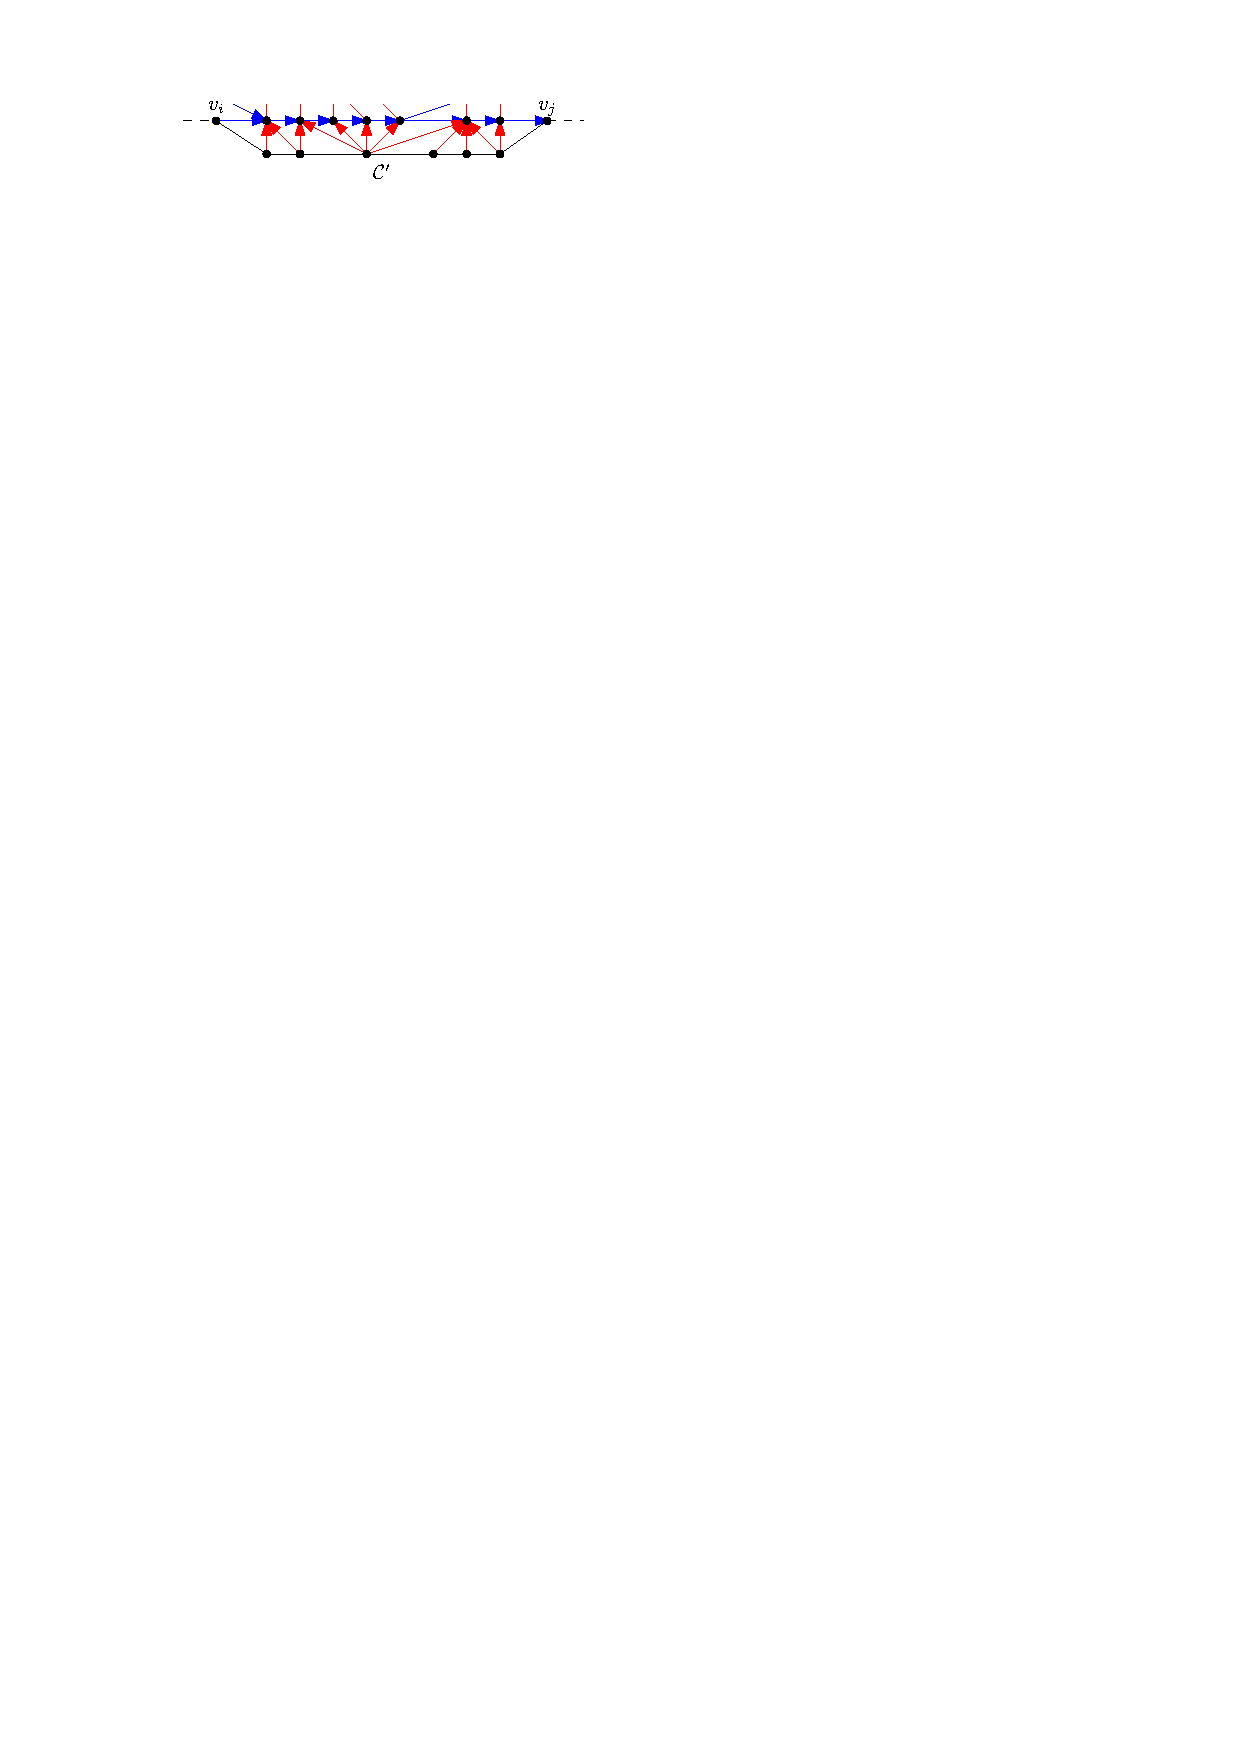
\includegraphics[width =\textwidth]{unifiedAlgo/img/sweep/updateAfter.pdf}
          \caption{After.}
      \end{subfigure}
      	\caption{The update.}
  \label{fig:sweep:update}
  \end{figure}


  \begin{lemma}
    \label{lm:sweep:updateMaintainsInvariants}
    Updating with a path $P'$ maintains all sweepcycle invariants.
  \end{lemma}
  \begin{proof}
    Invariant \ref{i:uni:SWandSE} remains true. Invariant \ref{i:uni:intVertCond} holds due to the way we colored the edges around the new interior vertices as can be seen in Figure~\ref{fig:sweep:update}.
    Furthermore, Invariant \ref{i:uni:redOutgoing} holds because every internal vertex of $P'$ has a left neighbor by Lemma \ref{lm:right:leftNeighborsOfTheRightNeighborPath}.

    To see that Invariants \ref{i:uni:noChords} and \ref{i:uni:no2Chords} hold, note that there can be no violating chords with both endpoints in the overlap of the old and new sweepcycle $\C \cap \C'$ by Invariants \ref{i:uni:noChords} and \ref{i:uni:no2Chords}.
    Since the updating path itself also has no violating chords (Lemma \ref{lm:sweep:augNoIregularity}),
    we know any violating chord $C$ has to have one vertex on $\P$ and one vertex on the unchanged part of old sweepcycle $\C \cap \C'$.
    However, these potential chords can not exist by Lemma \ref{lm:sweep:noConnectingIregularity}.
    Hence, $\C'$ is a valid new sweepcycle.
  \end{proof}

  If after the update the new sweepcycle $\C'$ has no interior vertices we terminate the algorithm,  this is described in Section~\ref{sss:terminating}.
  Otherwise, we start the update loop again by finding a new candidate path.

\subsubsection{Terminating the algorithm}
  \label{sss:terminating}
  When the sweepcycle has no more interior vertices, we can not update it anymore.
  However, at this point it is easy to color the remainder of the graph.
  All vertices in $\cpath$ must be adjacent to $\pS$ since $\pS \pW$ and $\pS \pE$ are part of $\C$ by Invariant \ref{i:uni:SWandSE}, $\cpath$ has no chords by Invariant \ref{i:uni:noChords} and $\C$ does not contain any interior vertices.
  All sweepcycle interior edges are adjacent to $\pS$, since otherwise we would have a chord in $\cpath$ (violating Invariant \ref{i:uni:noChords}).

  We color all interior edges of $\C$ red and orient them towards $\cpath$ and the edges in $\cpath$ are colored blue and oriented towards $\pE$. The termination step can be seen in Figure~\ref{fig:sweep:terminate}. This last move completes the interior vertex condition for vertices in $\C \sm {\pW, \pS, \pE}$ and also correctly completes the exterior vertex condition.


  \begin{figure}[b]
    \centering
    \begin{subfigure}[b]{0.45 \textwidth}
        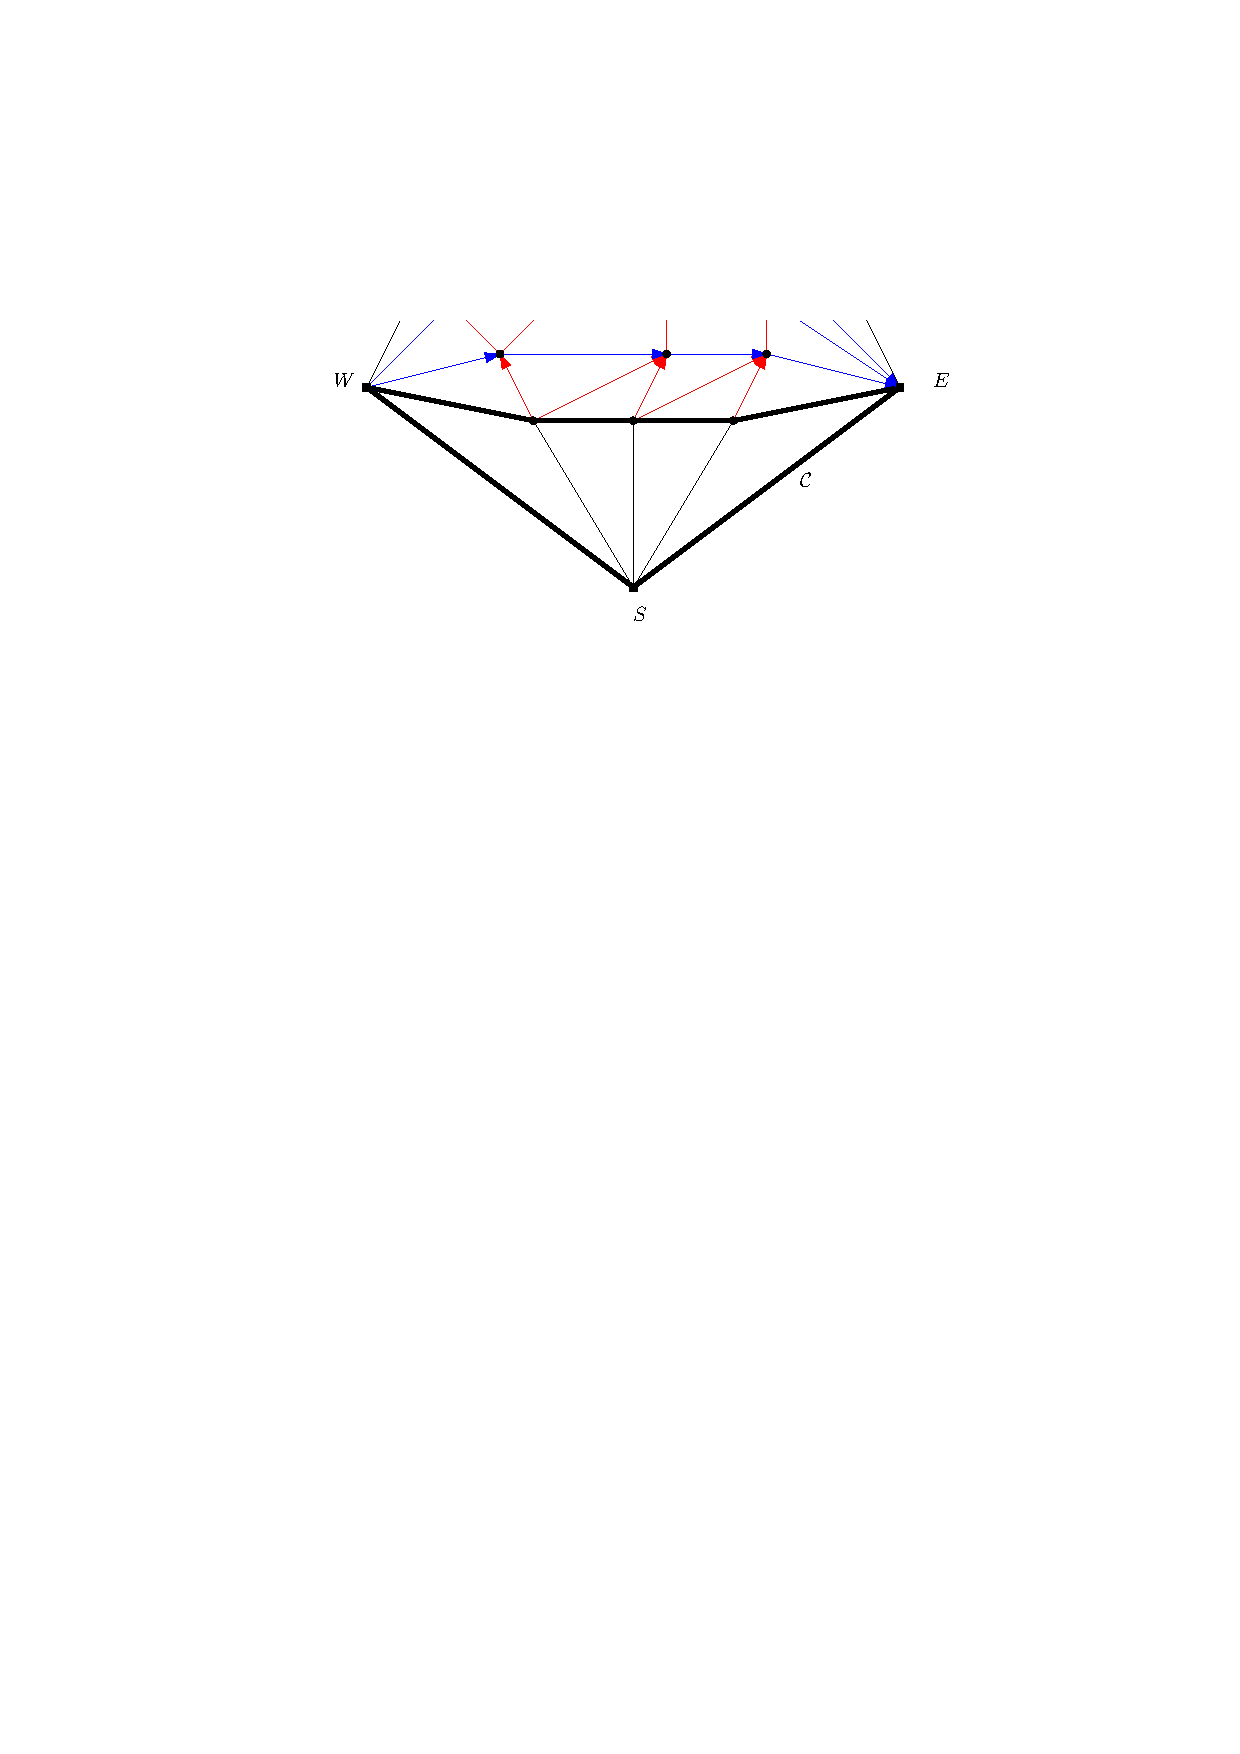
\includegraphics[width = \textwidth]{unifiedAlgo/img/sweep/terminateBefore.pdf}
        \caption{Before.}
    \end{subfigure}
    ~
    \begin{subfigure}[b]{0.45 \textwidth}
        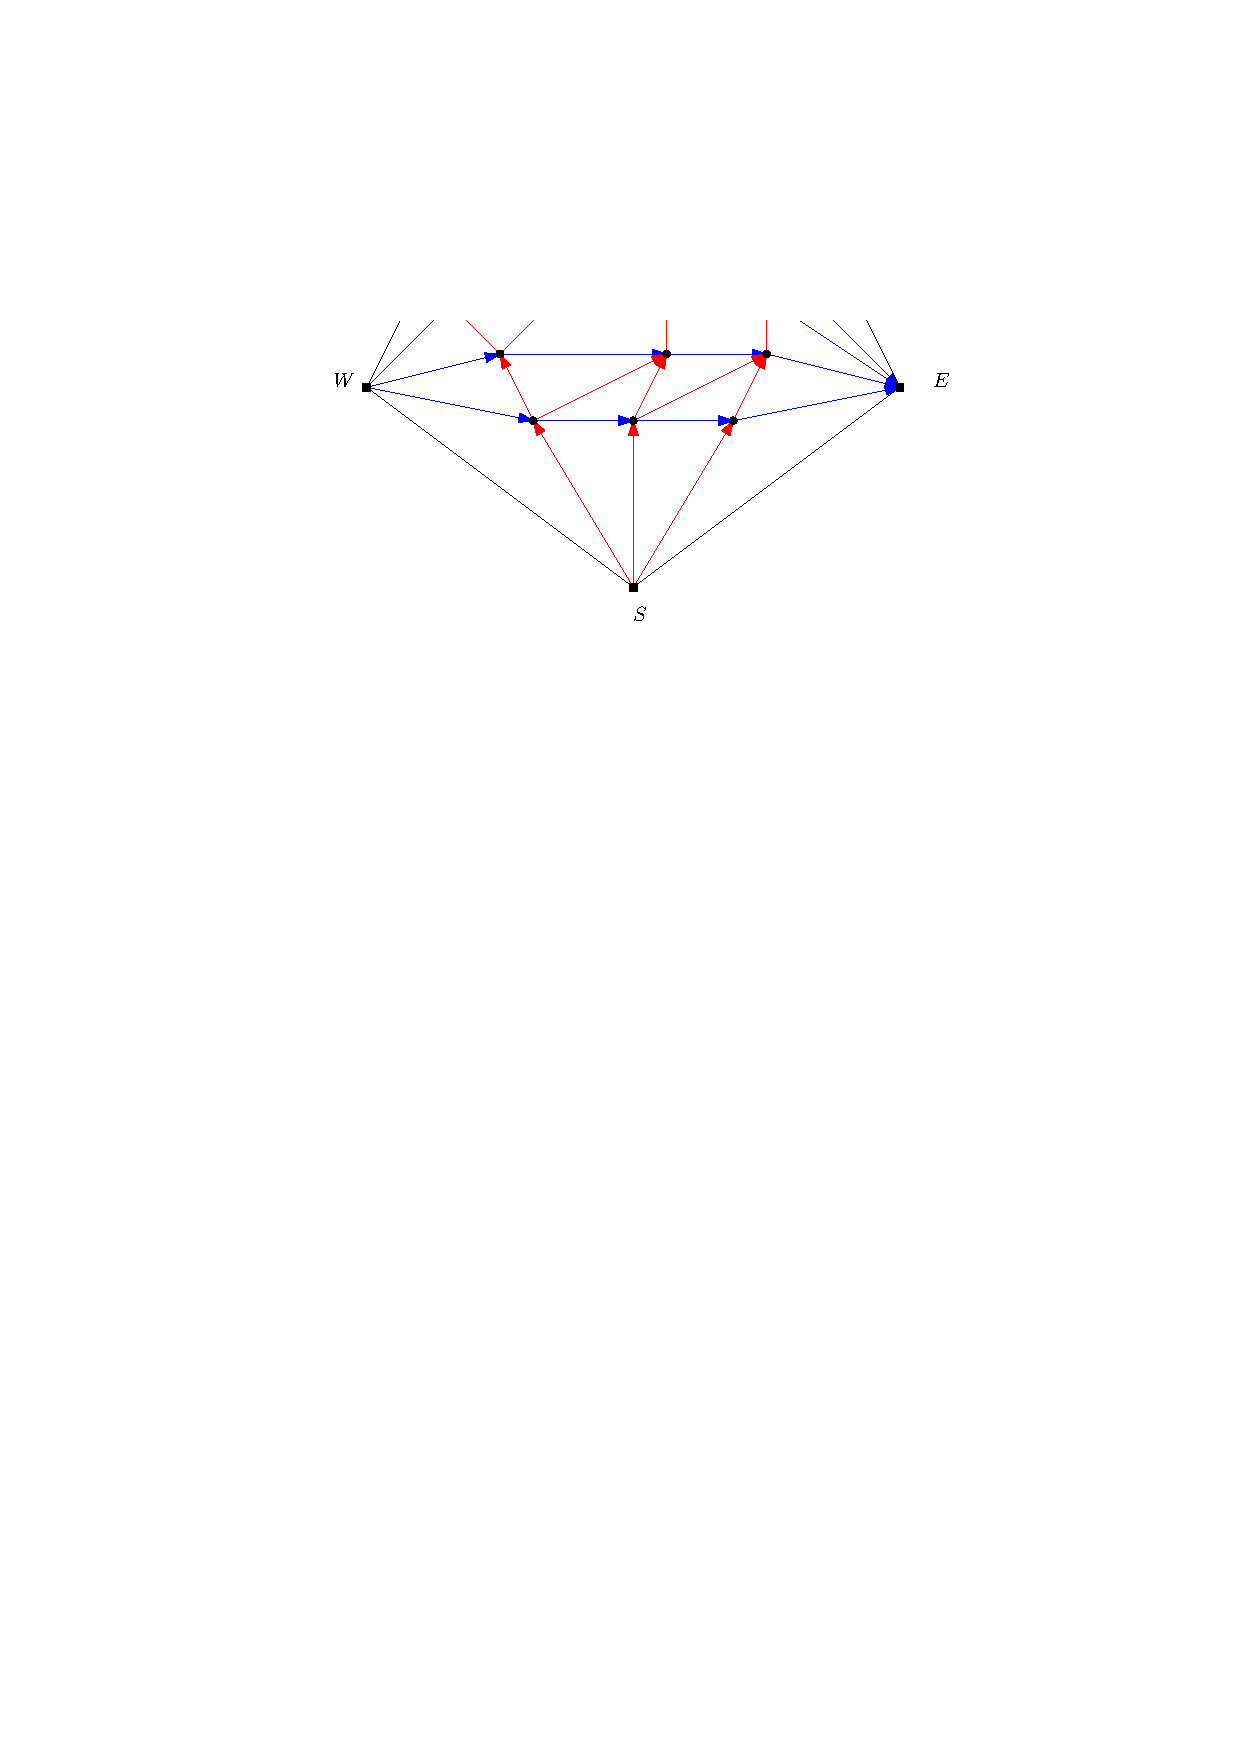
\includegraphics[width =\textwidth]{unifiedAlgo/img/sweep/terminateAfter.pdf}
        \caption{After.}
    \end{subfigure}
    \caption{The termination step.}
    \label{fig:sweep:terminate}
  \end{figure}

  \begin{lemma}
    \label{lm:sweep:REL}
    The resulting structure is a regular edge labeling
  \end{lemma}

  \begin{proof}
    After running the whole algorithm the interior vertex condition holds for all vertices in the graph by Invariant \ref{i:uni:intVertCond}. Furthermore, the poles are also colored correctly due to Invariant \ref{i:uni:SWandSE}.
  \end{proof}

\subsubsection{A useful property of this regular edge labelling}
  There still is a useful property of this regular edge labeling left to discuss (Lemma \ref{lm:sweep:NoTwoSplitsAboveEachOther}). Before we can state this property, we first need to introduce fans.

  \mypar{Fans}
    We want to better describe the interior of blue (or red) faces. Every interior edge of such face goes from one boundary path to the other (otherwise its start or end vertex would violate the interior vertex condition or create a face with a boundary path of length one violating Observation \ref{obs:rel:noBpOfLength1}). We now describe the edges from the split to the merge vertex of $F$.

    \begin{figure}[t]
      \centering
      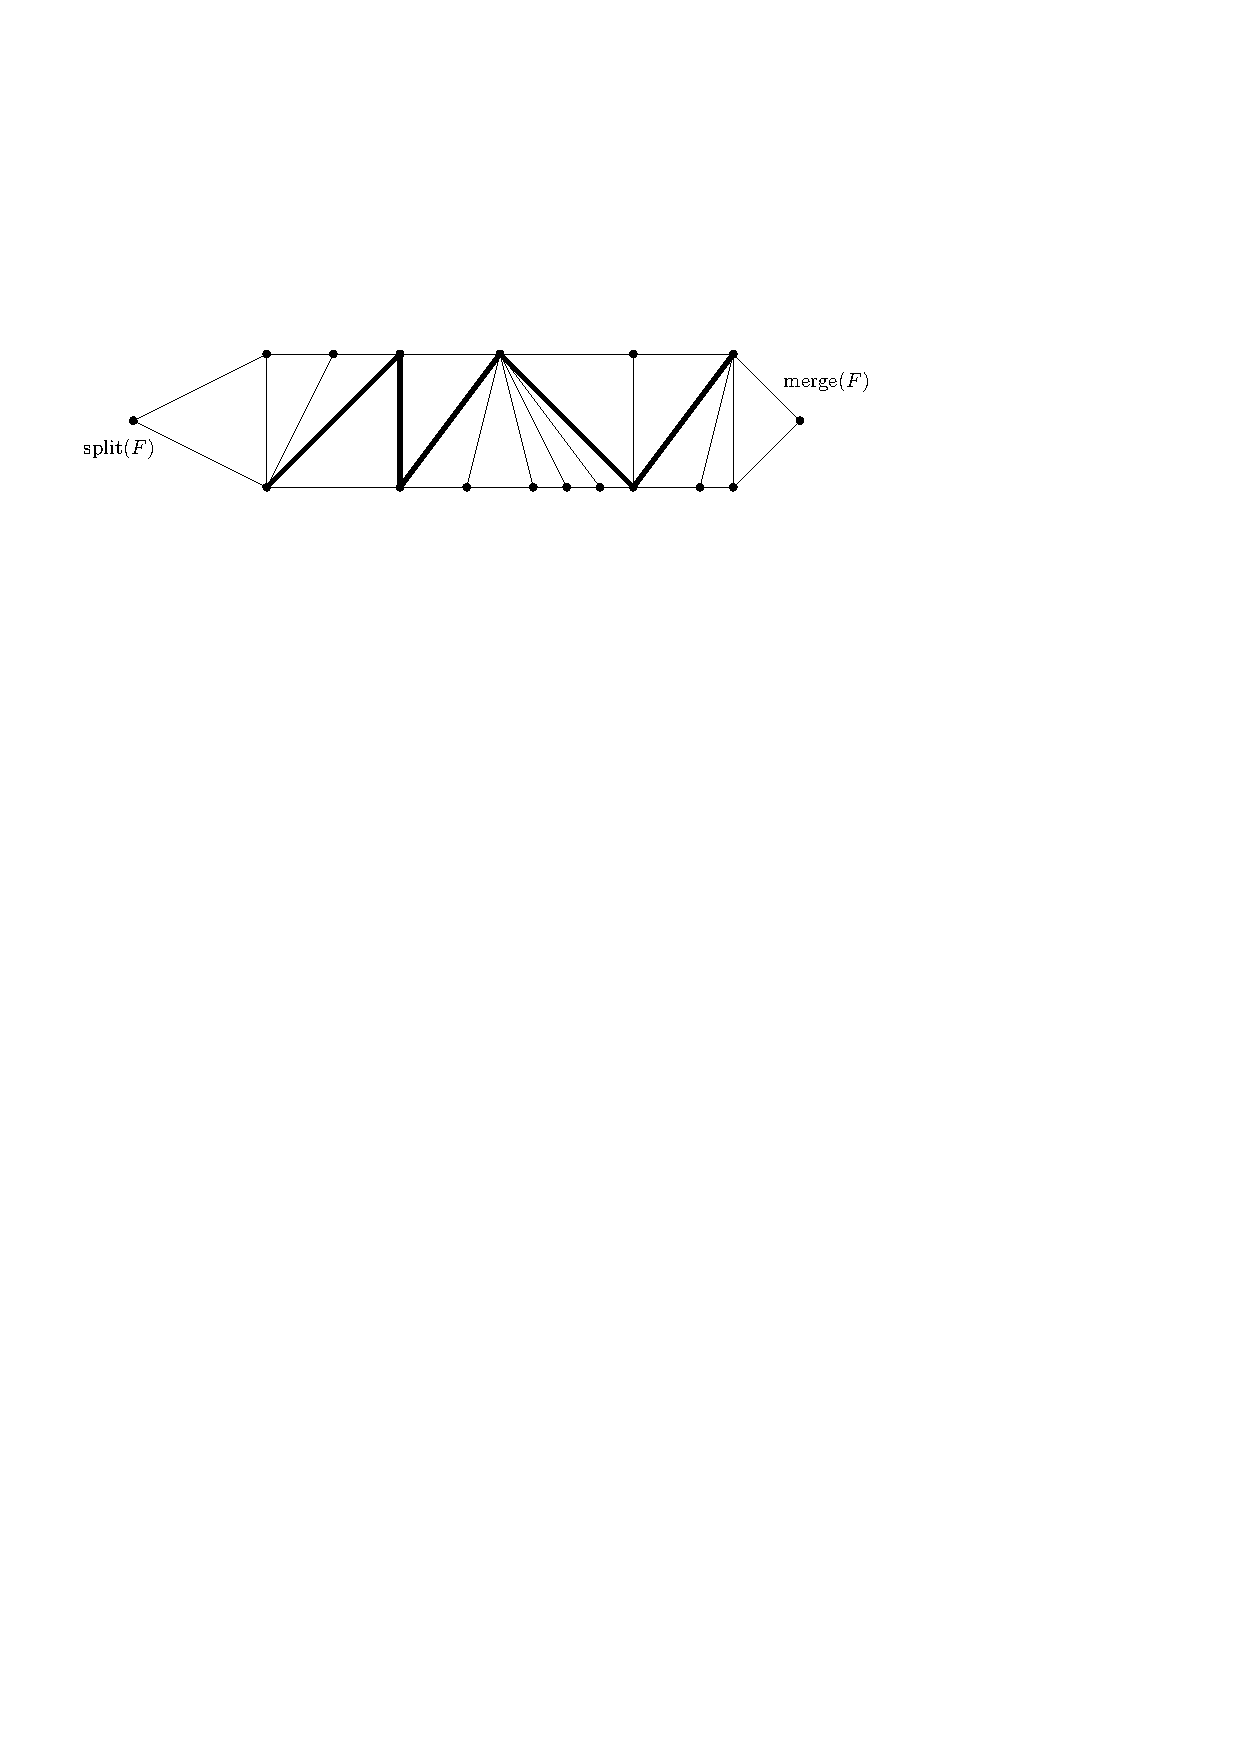
\includegraphics[scale=.9]{rectangularDuals/img/fans}
      \caption{An example face with fans.}
      \label{fig:uni:fans}
    \end{figure}

    Let $u_0 , u_1, \ldots u_n$ be the vertices of the top boundary path of $F$ and $v_0, v_1, \ldots, v_m$ the vertices of the bottom boundary path.
    That is $u_0=v_0$ is the split vertex and $u_n = v_m$ is the merge vertex.
    Since our graph is a triangulation, $u_1v_1$ must be an edge.
    For the second edge in the face we have two options, either $u_1v_2$ or $u_2v_1$, otherwise this edge and the previous one would not form a triangle.
    This argument holds for every subsequent edge, we can either increase the index of the top boundary path or the index of the bottom boundary path.
    Hence, this face is, for the readers that know this term, a \emph{triangle strip}.

    \begin{wrapfigure}{r}{7cm}
      \centering
      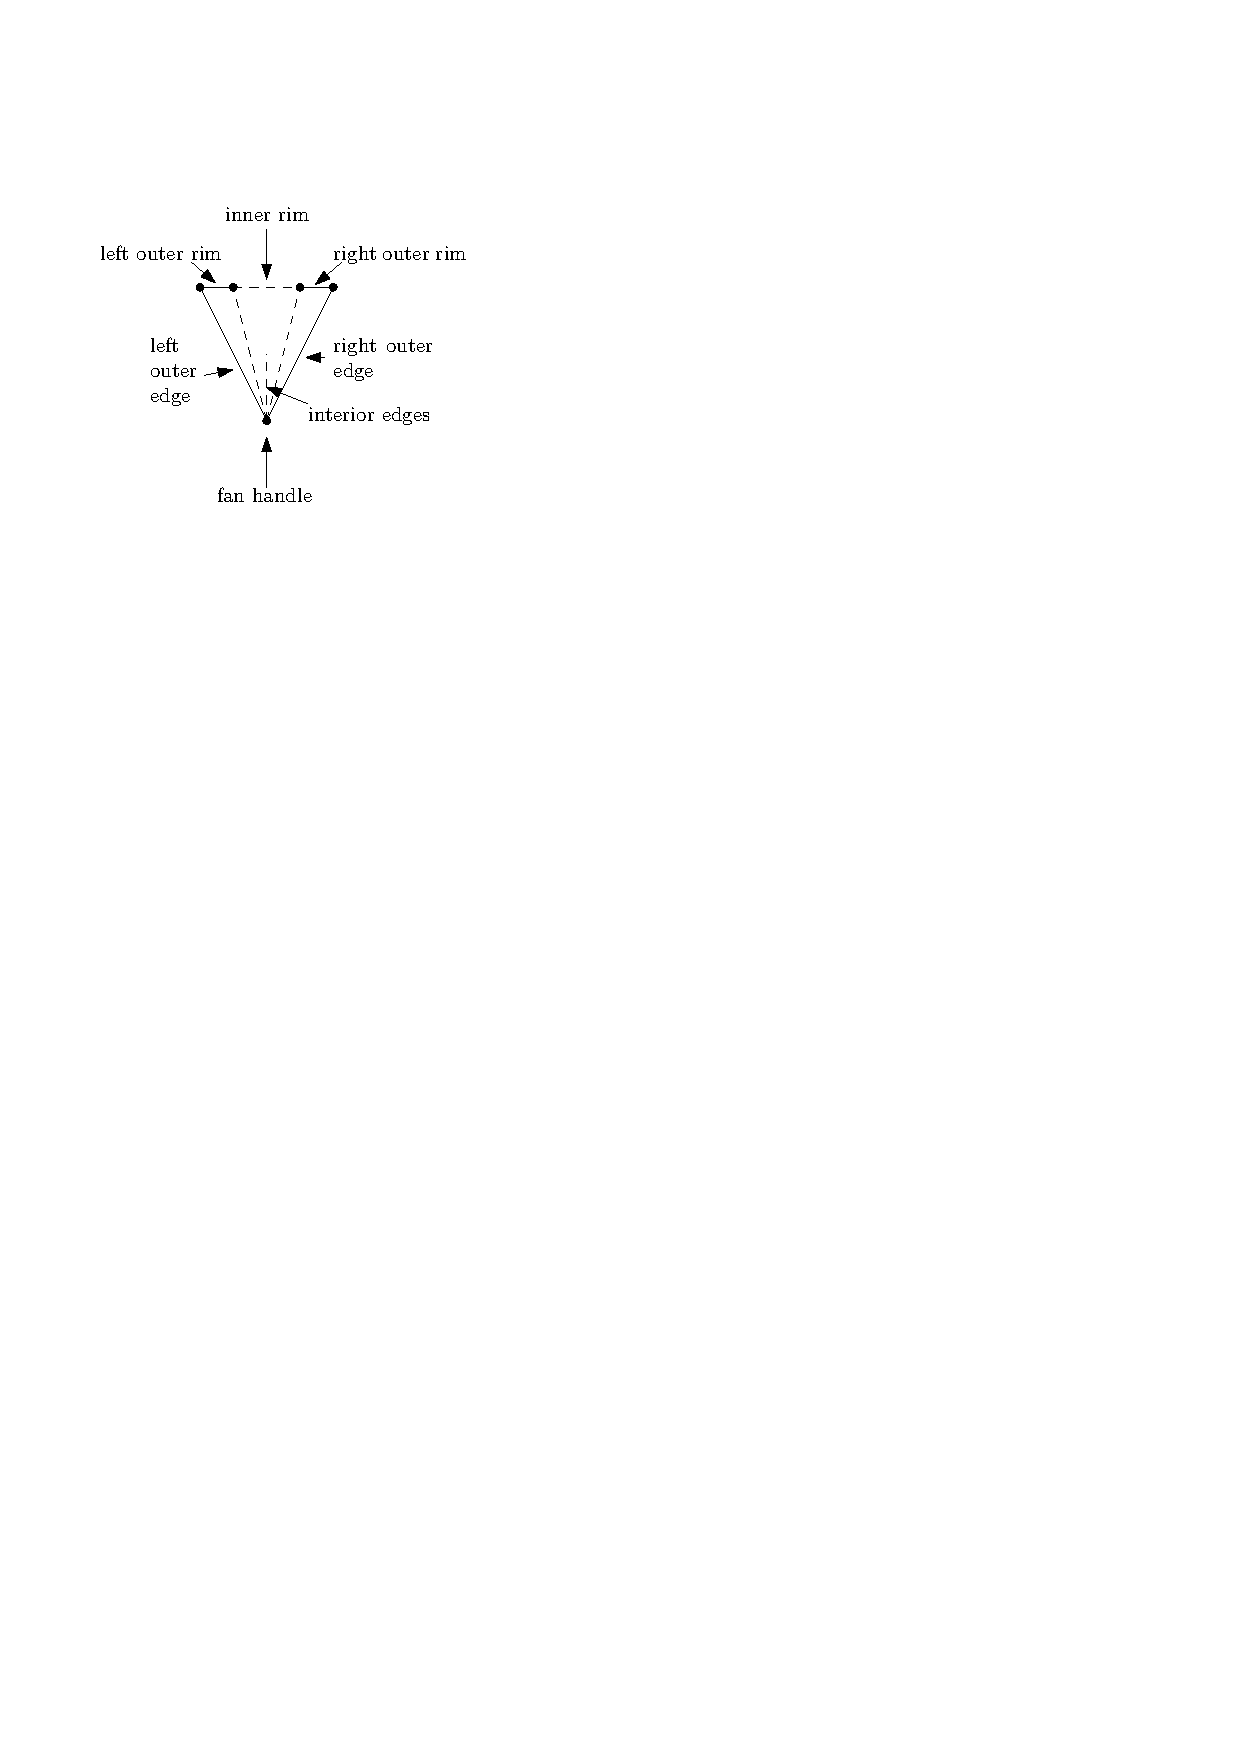
\includegraphics[scale=1]{rectangularDuals/img/fanterms}
      \caption{A number of fan-related terms.}
      \label{fig:rect:fanTerms}
    \end{wrapfigure}

    We call a maximal sequence of at least two edges increasing the index on the top boundary path (and thus keeping the index on the upper path fixed) a \emph{bottomfan} and a maximal sequence of at least two edges increasing the index on the bottom boundary path is called a \emph{topfan}.
    The \emph{size} of such a fan is the number of edges contained in the sequence. By the definition of a fan it has size of at least $2$.
    We use \emph{fans} to refer to both these \emph{types} of fans (i.e. topfans and bottomfans).
    We call a fan of size $3$ or larger a \emph{large fan} and a fan of size $2$ a \emph{small fan}.

    The \emph{left} of the fan is the part closest to the split vertex and the \emph{right} of the fan is the part closest to the merge vertex.

    In faces we alternately encounter bottomfans and topfans. If we would have two adjacent fans of the same type, we would just have a single larger fan of that type.
    In Figure~\ref{fig:uni:fans} we see a blue face consisting of subsequently a bottomfan of size $3$, a topfan of size 2, a bottomfan of size $2$, a topfan of size $6$, a bottomfan of size $3$ and a topfan of size $3$.

   We introduce some more terminology for fans: \emph{outer edges}, \emph{fan handles} and the \emph{rim} as can be seen in Figure~\ref{fig:rect:fanTerms}. The \emph{fan handle} $v$ is the vertex shared by all edges in the fan. Let $H$ be the induced subgraph of vertices incident to the edges in the fan. $H$ contains no edges not belonging to $F$ since these would lead to separating 3-cycles. The \emph{rim} is the path given by $F\sm{v}$.
   The \emph{outer rim} are the two extreme edges of this path and the \emph{outer edges} are the edges between the fan handles and the extreme vertices of the \emph{rim}.

   A similar discussion can be given for red faces. However then we have \emph{right fans} and \emph{left fans} instead of bottom and top fans.

\newpage\fxerror{check this new page}
  \mypar{The property}

    \begin{wrapfigure}{!r}{5cm}
      \centering
      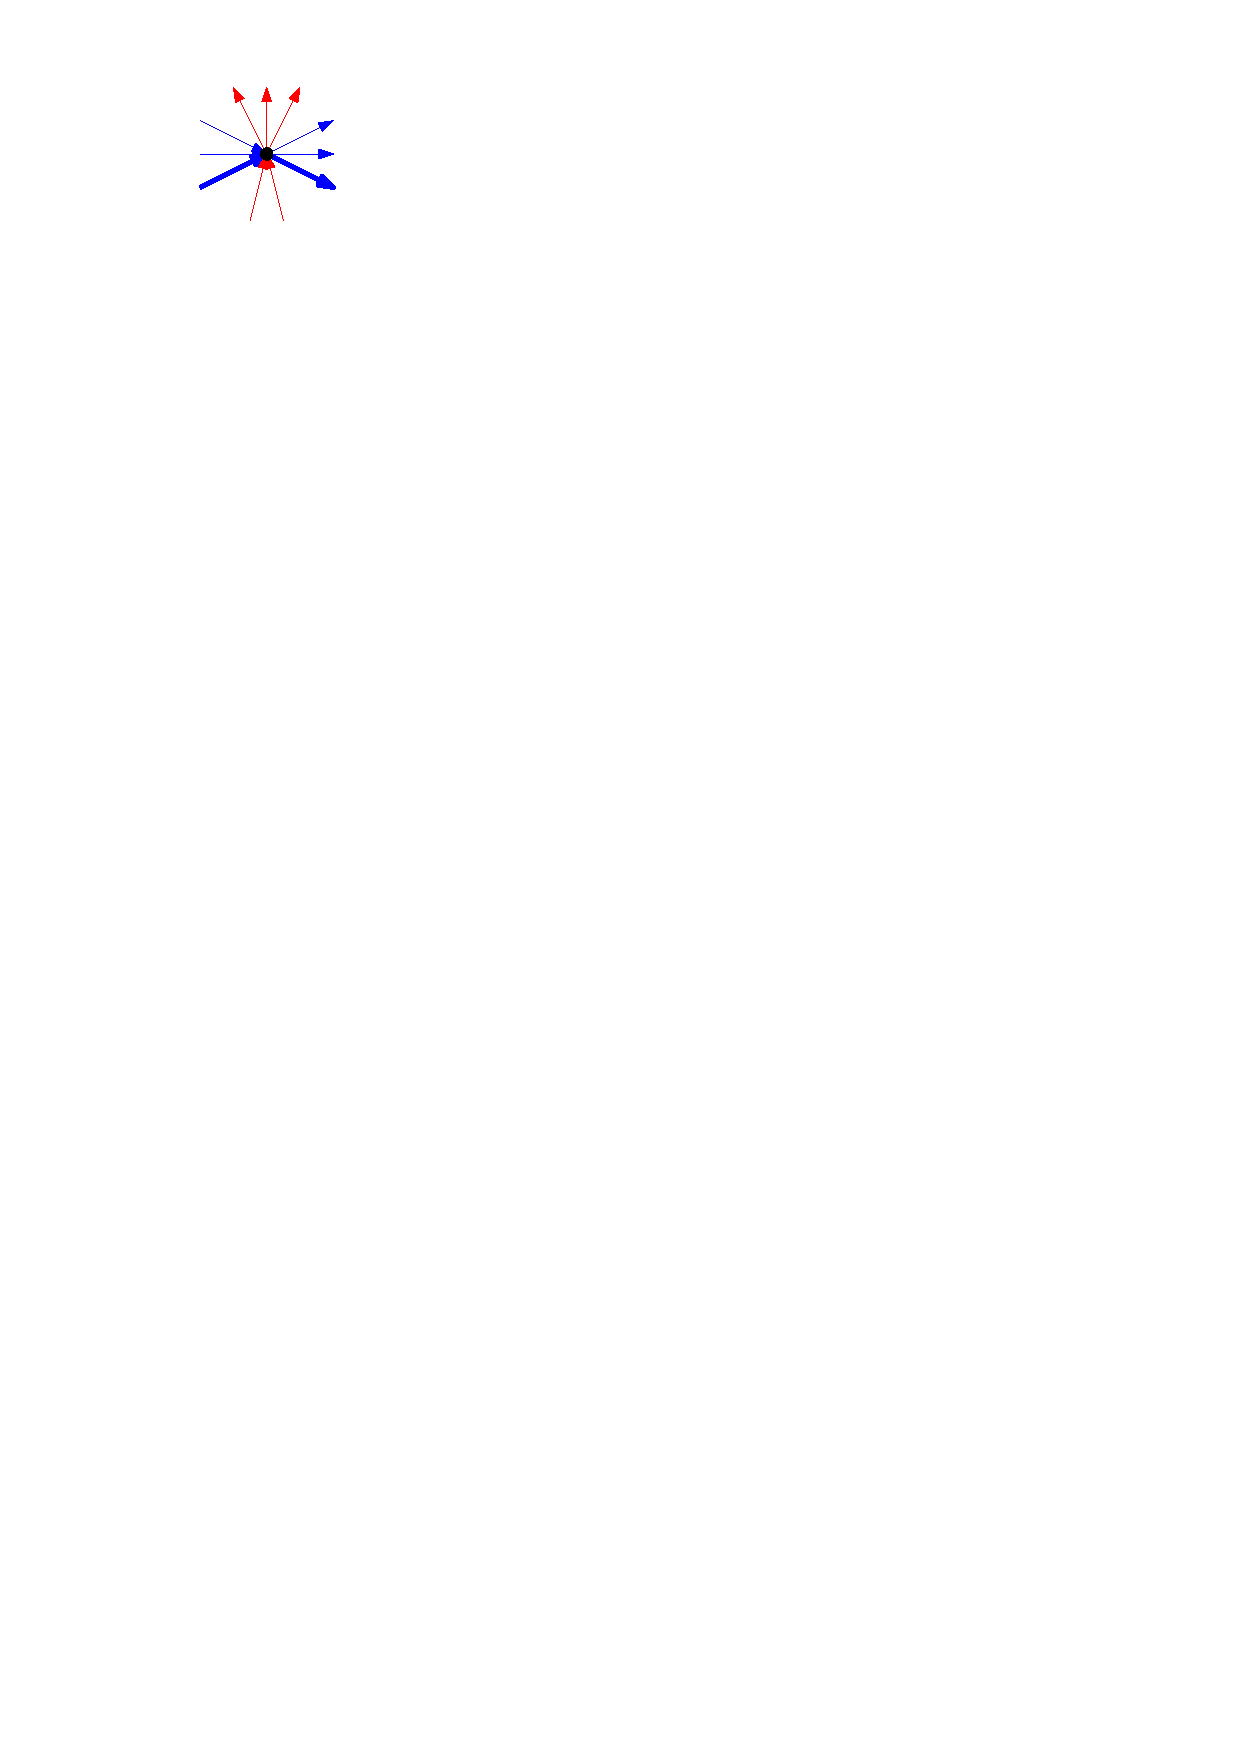
\includegraphics[scale=.9]{unifiedAlgo/img/sweep/bottompath.pdf}
      \caption{The bottom path of this splitvertex is given in bold.}
      \label{fig:sweep:bottomPath}
    \end{wrapfigure}

    Before finally discussing the property, we introduce two more definitions.
    A \emph{splitvertex} is a vertex with more than one outgoing blue edge.
    Given a splitvertex $v$, the \emph{bottom} path is the path that comes in trough the first edge in the interval of incoming blue edges in the rotation at $v$ and leaves through the last edge in the interval of outgoing blue edge in the rotation at $v$.
    See Figure~\ref{fig:sweep:bottomPath}.

    \begin{lemma}
      \label{lm:sweep:NoTwoSplitsAboveEachOther}
      Let $v$ be any splitvertex. Then the subsequent vertex on the bottom path $w$ can not be the handle of a large topfan.
    \end{lemma}

    \begin{proof}
      There are two possible causes of $v$ being a splitvertex, $v$ is either adjacent to $\pS$ or $v$ is a splitvertex due to a chord.

      If $v$ is a splitvertex because it is adjacent to $\pS$ then since $w$ is on the bottom path it also has to be adjacent to $\pS$ by the definition of the bottom path.
      Hence, $w$ is not the handle of a large topfan.

      If $v$ is a splitvertex due to a chord $v a b x$ we can continue the bottom path past $w$ as a bottom path that eventually goes to $x$ since every chord is evaded by a single path from $v_k$ to $v_\ell$ in the algorithm.
      We denote this extended bottom path by $\P$.
      The situation is depicted in Figure~\ref{fig:sweep:botomPathChord}.

      The interior of  $vabx \oplus \rev \P$ has no vertices. Suppose there would be such a vertex . Then, since $\P$ is a bottom path the blue path going trough this vertex has to start at $a$ and end at $b$. But this gives a blue face with only one edge on its bottom boundary path violating Observation \ref{obs:rel:noBpOfLength1}. Since our graph is a regular edge labeling, $vabx \oplus \rev \P$ has no interior vertices.

      This also implies all interior edges are red (by the definition of bottom path) and thus that $ab$ is blue otherwise we would get a monochromatic triangle.

      Now $w$ can not be connected to any vertex in $\P$ since that would again give a face with a boundary path of length 1 (Observation \ref{obs:rel:noBpOfLength1}).
      So $w$ can only be connected to $a$ and $b$ and is thus a topfan of size at most $2$.
      (If it is a topfan at all, since we do not consider topfans of size 1 as topfans.)
    \end{proof}

    \quad
    \quad
    \begin{figure}[h]
      \centering
      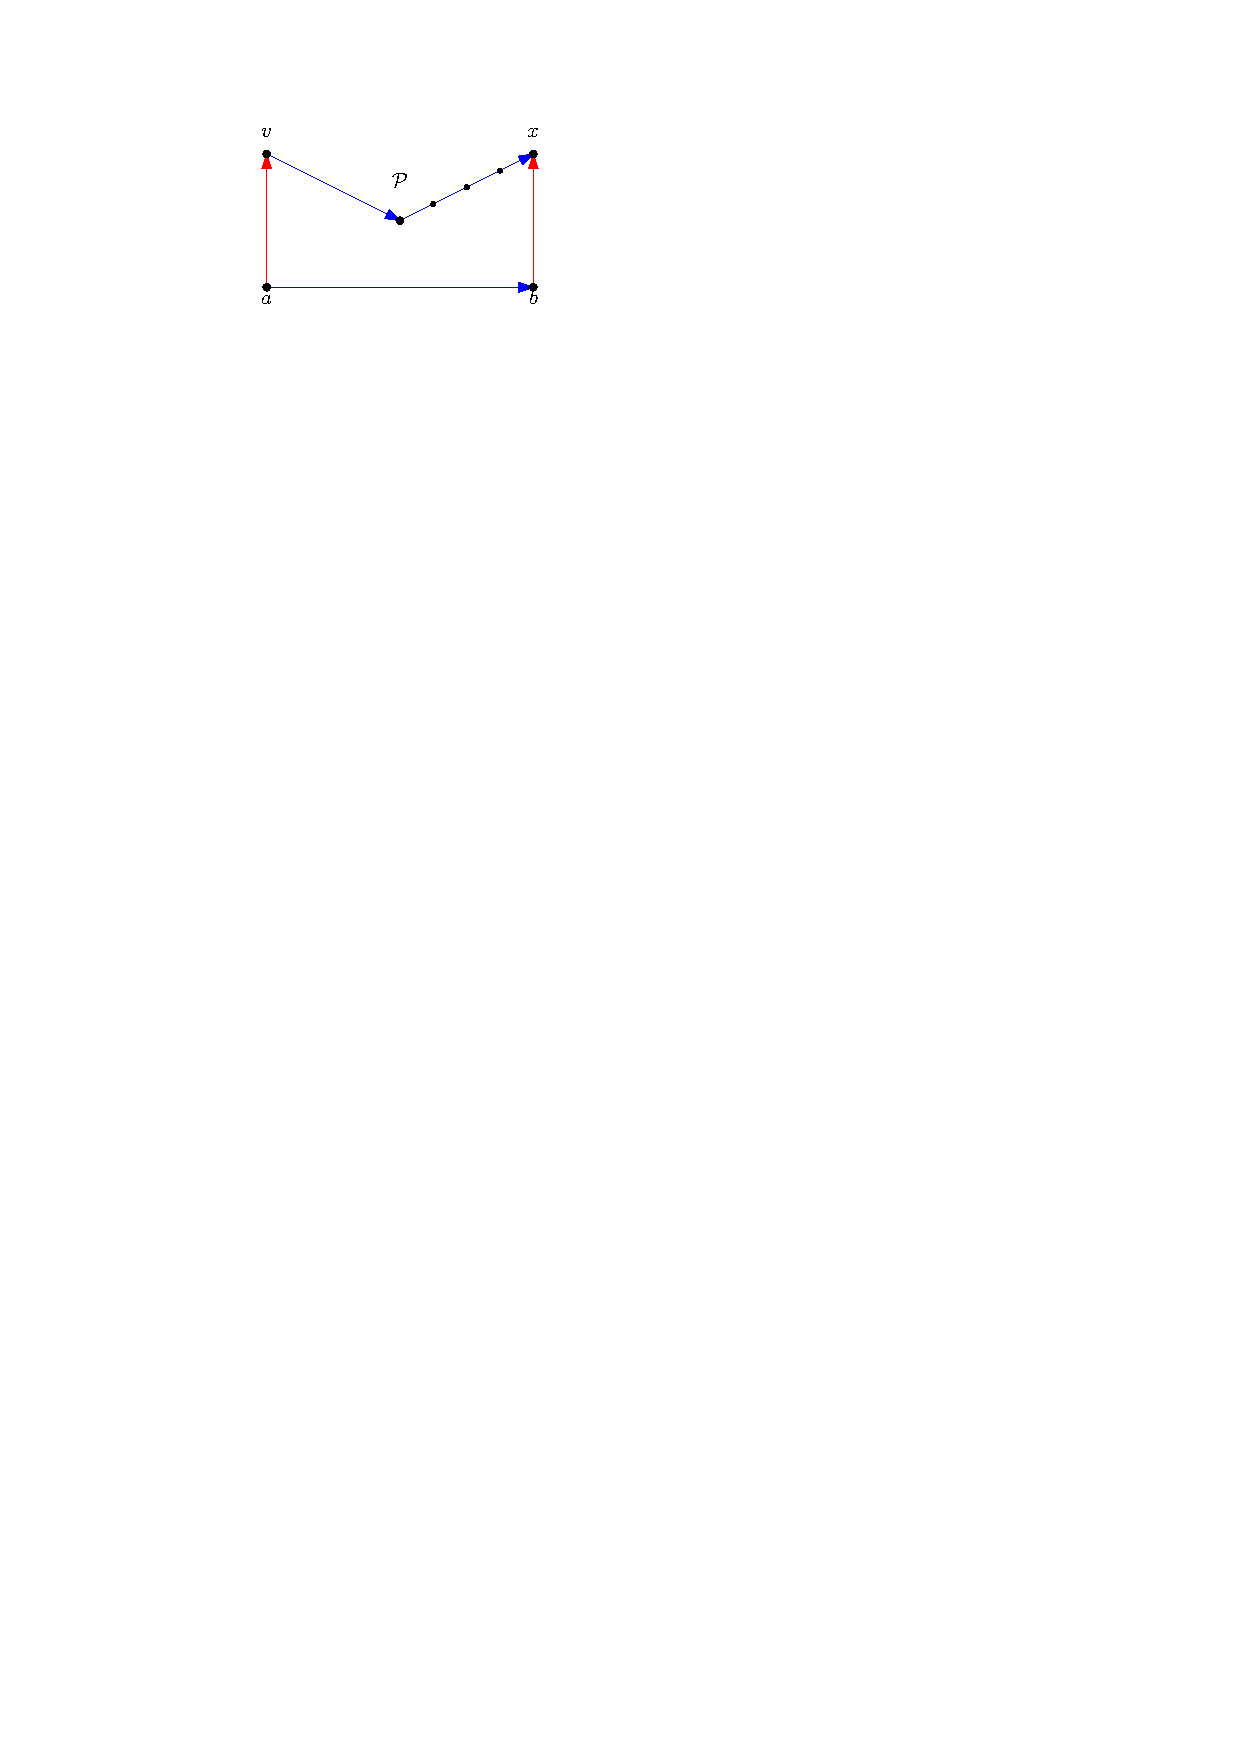
\includegraphics[scale=1]{unifiedAlgo/img/sweep/bottompathChord.pdf}
      \caption{The situation in the proof of Lemma \ref{lm:sweep:NoTwoSplitsAboveEachOther}.}
      \label{fig:sweep:botomPathChord}
    \end{figure}
